%% LyX 2.1.4 created this file.  For more info, see http://www.lyx.org/.
%% Do not edit unless you really know what you are doing.
\documentclass[11pt,a4paper,polish,thesis]{dcsbook}
\usepackage[utf8]{inputenc}
\setcounter{secnumdepth}{3}
\usepackage{color}
\usepackage{babel}
\usepackage{array}
\usepackage{longtable}
\usepackage{multirow}
\usepackage{graphicx}
\usepackage[unicode=true,pdfusetitle,
 bookmarks=true,bookmarksnumbered=true,bookmarksopen=true,bookmarksopenlevel=1,
 breaklinks=true,pdfborder={0 0 0},backref=false,colorlinks=true]
 {hyperref}
\hypersetup{
 urlcolor=linkcolor,linkcolor=linkcolor,citecolor=linkcolor}

\makeatletter

%%%%%%%%%%%%%%%%%%%%%%%%%%%%%% LyX specific LaTeX commands.
\pdfpageheight\paperheight
\pdfpagewidth\paperwidth

%% Because html converters don't know tabularnewline
\providecommand{\tabularnewline}{\\}

%%%%%%%%%%%%%%%%%%%%%%%%%%%%%% Textclass specific LaTeX commands.
\RequirePackage{dcslib}[2012/01/30]

%%%%%%%%%%%%%%%%%%%%%%%%%%%%%% User specified LaTeX commands.
%
%  $Id: thesis-template.lyx,v 1.7 2011/12/22 12:10:18 sobaniec Exp $
%

\makeatother

\usepackage{listings}
\renewcommand{\lstlistingname}{\inputencoding{latin2}Listing}

\begin{document}

\author{Wojciech Mioduszewski}


\title{Klasyfikacja danych opisanych za pomocą szeregów czasowych}


\date{Poznań, 2015}


\supervisor{dr inż. Jerzy Błaszczyński}

\maketitle


\frontmatter

\tableofcontents{}

\mainmatter


\chapter{Wstęp}


\section*{Cel i zakres pracy}

Cel: Opracowanie i implementacja różnych podejść do klasyfikacji danych
czasowych. \\
Zadania: 
\begin{itemize}
\item Zapoznać się z literaturą tematu.
\item Opracować wybrane podejścia do klasyfikacji danych czasowych.
\item Zaimplementować i udokumentować zaproponowane rozwiązania.
\item Przeprowadzić eksperyment obliczeniowy
\end{itemize}
Początkowo celem niniejszej pracy była analiza szeregów czasowych
zawierających dane ciśnienia w oku pacjentów zdrowych, oraz tych ze
zdiagnozowaną jaskrą. Ponadto zamiarem było użycie do tego celu metody
SAX, a następnie zbudowanie klasyfikatora potrafiącego sklasyfikować
dane wytworzone przez tą metodę. Następnie, aby nie testować sposobów
klasyfikacji tylko i wyłącznie na danych zebranych w celu oceny jaskry,
lecz również sprawdzić jak wybrane i stworzone metody poradzą sobie
w odniesieniu do innych szeregów czasowych, rozszerzono zbiór danych
o kolejne zestawy szeregów czasowych. Kolejną rzeczą, od której należało
się uniezależnić są klasyfikatory, dlatego też eksperymenty przeprowadzone
zostały z wykorzystaniem różnych typów klasyfikatorów.

Ostatecznie po wielu testach wyklarowano sześć eksperymentów, których
wyniki porównano i zinterpretowano. Składowe każdego z eksperymentów
zostały dokładnie opisane. 

W rozdziale 2 przedstawiono kilka podejść analizy szeregów czasowych
wybranych z przeanalizowanej literatury. Ponadto zademonstrowano działanie
dwóch kluczowych algorytmów rozważanych w tej pracy, to jest algorytmu
SAX oraz DTW. Rozdział 3 poświęcono zobrazowaniu koncepcji projektu,
toteż rozdział ten skupia się na przestudiowaniu różnych sposobów
przetwarzania danych jeszcze zanim te trafią do klasyfikatora. Czytelnik
znajdzie tu również krótki opis użytych klasyfikatorów, a także miary
jakie użyto do oceniania dokładności klasyfikacji. 

Rozdział 4 przedstawia sposób implementacji programu potrzebnego do
przeprowadzenia eksperymentów. Zamieszczono tutaj zwięzłe opisy użytych
bibliotek, oraz szczegółowy opis importu oraz eksportu danych - tak
aby w przyszłości nie było problemu z ewentualnym rozszerzeniem istniejącego
kodu. Rozdział 5 zawiera analizę wyników oraz wnioski, a tym samym
stanowi podsumowanie niniejszej pracy.


\chapter{Kontekst teoretyczny}


\section{Definicja szeregu czasowego}

Szereg czasowy jest to seria pewnych obserwacji osadzonych w czasie.
Można powiedzieć, że jest to przyporządkowanie danych liczbowych do
odpowiadających im punktów w czasie, najczęściej z jednakowymi odstępami
między kolejnymi wartościami\cite{Stefan}.


\section{Przykładowe metody analizy danych czasowych\cite{Shum2010}}

Tak obszerny problem jak analiza danych czasowych musi nieść za sobą
rozmaite metody przeprowadzania tej analizy. Wprawdzie do ostatecznego
eksperymentu wybrano tylko dwie z nich - regresję oraz DTW, to postanowiono
przedstawić pokrótce czym charakteryzują się poszczególne metody oraz
ewentualnie dlaczego zostały porzucone.


\subsection{Regresja liniowa\cite{StefanRegresja}}

Regresja w odniesieniu do danych czasowych sprowadza się do estymowania
liniowego trendu jaki prezentuje badany szereg. Koncepcyjnie metoda
polega na stworzeniu funkcji liniowej, która w najbardziej dokładny
sposób przybliża wartości na kolejnych obserwacjach. Matematyczny
model regresji ma zatem następującą postać: 
\[
y=ax+b
\]
Jako miarę błędu przyjmuje się sumę kwadratów różnicy między oszacowaniami,
a wartościami właściwymi.
\[
S=\sum_{i=1}^{n}(y_{i}-\hat{y_{i}})^{2}
\]



\subsection{Wygładzanie (ang. smoothing)}

Wygładzanie to metoda starająca się zniwelować ponadprzeciętne różnice
wartości między kolejnymi pomiarami. Dzięki temu podejściu można dokładniej
przyjrzeć się ogólnemu zarysowi funkcji, czy jej okresowymi trendami,
kosztem precyzji. Podejście to pozwala zminimalizować ewentualne szumy
z badanego zbioru. Metoda ta jako argument przyjmuje szerokość okna
$k$, w ramach którego będą uśredniane wartości. W pierwszym kroku
liczy się średnią z $k$ pierwszych wartości szeregu, następnie przesuwa
okno o jeden element i znów liczy średnią z $k$ wartości. Wyjściowy
zbiór dla $n$-elementowego zbioru będzie miał $n-k$ wartości.

Poniżej dla porównania zaprezentowano wykres miary TFADJ w przeciągu
doby \ref{fig:Czysty-sygna=000142-TFADJ}, oraz jego wygładzony odpowiednik
\ref{fig:Wyg=000142adzony-sygna=000142-TFADJ}. Jak widać operacja
wygładzania zredukowała skrajne wychylenia szeregu i wyklarowała paraboliczną
tendencję tego zbioru.

\begin{figure}[tbph]
\includegraphics[width=15cm]{\string"figures/Clean 15 D1\string".jpg}\caption{Czysty sygnał TFADJ\label{fig:Czysty-sygna=000142-TFADJ}}
\end{figure}


\begin{figure}[tbph]
\includegraphics[width=15cm]{\string"figures/Smooth 15 D1\string".jpg}

\caption{Wygładzony sygnał TFADJ\label{fig:Wyg=000142adzony-sygna=000142-TFADJ}}
\end{figure}



\subsection{Modele ARIMA}

Model ARIMA (ang. Autoregressive Integrated Moving Average) koncepcyjnie
składają się z trzech części - jest to autoregresja, integracja oraz
średnia ruchoma. 

Autoregresja jest to metoda, która skupia się na wyrażeniu bieżącej
wartości na podstawie$n$ poprzednich. Dla przykładu, funkcja dla
$n=2$ wygląda w ten sposób:
\[
x_{t}=\omega_{t-2}x_{t-2}-\omega_{t-1}x_{t-1}+\omega_{t}
\]


Średnia ruchoma ideowo jest bardzo zbliżona do autoregresji, jednak
skupia się na zaburzeniach (ang. lags) w szeregu, a nie bezpośrednio
na wartościach. Wzór przedstawia się analogicznie jak w autoregresji.

Integracja z kolei pozwala na zastosowanie modelu ARIMA do procesów
niestacjonarnych, które da się sprowadzić do procesów stacjonarnych
dzięki przekształceniu oryginalnego sygnału na różnice (ang. difference
equations) pomiędzy wartością obecną, a poprzednią. 

Podsumowując, modele ARIMA doskonale spisują się w prognozowaniu wartości,
bazując na danych historycznych szeregu, jednak nie są najlepszym
wyborem jako metoda klasyfikacji. Ponadto metoda nie jest najłatwiejsza
matematycznie. Biorąc pod uwagę te argumenty, metoda ta została odrzucona.


\subsection{Analiza spektralna (widmowa)}

Celem analizy spektralnej (ang. spectral analysis) szeregów czasowych
jest zidentyfikowanie najczęściej powtarzających się wzorców w czasie,
a następnie przybliżenie danego szeregu do procesu okresowego określonego
wzorem:
\[
x_{t}=U_{1}\cos(2\Pi\omega t)+U_{2}\sin(2\Pi\omega t)
\]
gdzie amplituda funkcji to $A=\sqrt{U_{1}^{2}+U_{2}^{2}}$. 

Jak widać jest to kolejna metoda, za którą stoi solidne matematyczne
zaplecze i która wymierzona jest w szeregi cykliczne, z którymi w
zbiorze danych pacjentów jaskry nie mamy do czynienia, zatem metodę
tę odrzucono.


\section{SAX (Symbolic Aggregate approXimation)}

Już na początkowym etapie rozważań nad zakresem niniejszej pracy zadecydowano,
że jednym głównych nurtów jaki przyjmie, będzie przekształcanie sygnału
według metody SAX. Mówiąc pokrótce, jest to metoda odzwierciedlająca
oryginalny sygnał w ciąg znaków, co stwarza możliwości klasyfikacji
danych za pomocą istniejących już algorytmów tekstowych.


\subsection{Założenia}

Korzystając z pomysłu prof. Eamonna przyjęto założenie, że dla szeregów
czasowych o równych odstępach czasowych między pomiarami, można pominąć
dane dotyczące momentu, w którym pomiaru dokonano i uprościć ten szereg
do sekwencji samych wartości. W następujących rozdziałach przyjęto
że operuje się na zbiorze $N$-elementowym o postaci $x_{1},x_{2},\ldots,x_{n}$


\subsection{Schemat działania}

Stworzenie reprezentacji SAX dla szeregu czasowego składa się z trzech
etapów:


\subsubsection{Z-normalizacja szeregu czasowego}

Na potrzeby przedstawienia wzoru dla odchylenia standardowego przyjęto
następującą definicję sumy elementów zbioru:
\[
s_{j}=\sum_{k=1}^{N}x_{k}^{j}
\]
dzięki któremu można przedstawić wzór na odchylenie standardowe tak
jak poniżej\cite{FormulaStdDeviation}:
\[
std=\sqrt{\frac{Ns_{2}-s_{1}^{2}}{N(N-1)}}
\]
Mając obliczone odchylenie standardowe i średnią wartość dla zbioru,
którą wyrażono poniżej symbolem $mean$ można przejść do właściwej
normalizacji, co oznacza przekształcenie każdego z elementów zbioru
w sposób przedstawiony poniżej:
\[
x_{i}=\frac{x_{i}-mean}{std}
\]



\subsubsection{Dyskretyzacja sygnału za pomocą algorytmu PAA (Piecewise Aggregate
Approximation)}

Jednym z argumentów, jaki przyjmuje algorytm SAX jest długość łańcucha
wyjściowego - co w praktyce sprowadza się do tego na ile części podzielić
długość szeregu czasowego. Oznacza to, że metoda zmniejsza wymiarowość
szeregu z $N$ do żądanych $M$ elementów. Przebieg algorytmu jest
intuicyjny - sekwencja $x_{1},x_{2},\ldots,x_{N}$transformowana jest
do postaci $y_{1}y_{2},\ldots,y_{M}$ poprzez podział sekwencji $N$-elementowej
na $M$ równych części według wzoru\cite{SaxFundamentals}:
\[
y_{i}=\frac{M}{N}\sum_{j=\frac{N}{M}(i-1)+1}^{(N/M)i}
\]
Poniżej przedstawiono przykładową dyskretyzację dla następującego
szeregu czasowego:

\begin{tabular}{|c|c|c|c|c|c|c|c|c|c|c|}
\hline 
i & 1 & 2 & 3 & 4 & 5 & 6 & 7 & 8 & 9 & 10\tabularnewline
\hline 
oryginalny sygnał $x_{i}$ & 2 & 6 & 3 & 9 & 10 & 9 & 2 & 1 & 7 & 4\tabularnewline
\hline 
\end{tabular}

dzieląc szereg dziesięcioelementowy na pięć równych części algorytmem
PAA\cite{PaaGithub}:
\begin{figure}[tbph]
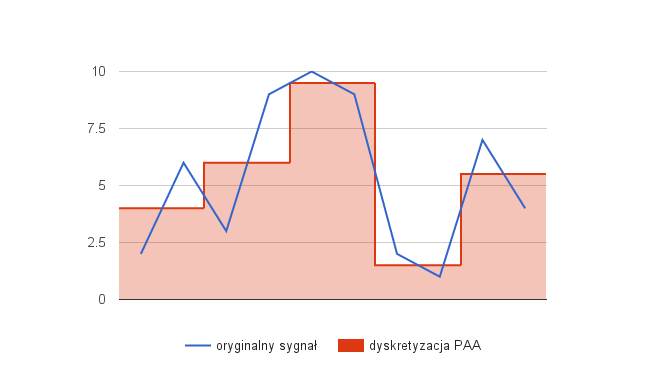
\includegraphics[width=15cm]{figures/paa_moje}

\caption{Porównanie oryginalnego szeregu czasowego i jego 5-elementowej dyskretyzacji}


\end{figure}
Dzięki temu otrzymano redukcję pięciowymiarową:

\begin{tabular}{|c|c|c|c|c|c|}
\hline 
i & 1 & 2 & 3 & 4 & 5\tabularnewline
\hline 
zdyskretyzowany sygnał $y_{i}$ & 4 & 6 & 9.5 & 1.5 & 5.5\tabularnewline
\hline 
\end{tabular}


\subsubsection{Algorytm SAX}

Jak wspomniano wyżej, jednym z argumentów jakie przyjmuje algorytm
SAX jest długość sekwencji wyjściowej, zaś drugim - liczba dostępnych
liter w alfabecie. Ta liczba precyzuje na ile części podzielić zbiór
wartości danego (przetworzonego już) szeregu, a tym samym jakie indeksy
(znaki) przypisać wartościom lądującym w poszczególnych zakresach.
Do przypisania znaków dla odpowiednich przedziałów potrzebny jest
przedział danych zatem obliczyć różnicę między elementem minimalnym
a maksymalnym zbioru $y$ 
\[
d=|max(y)-min(y)|
\]
a następnie ustalić krok $k$, ustalający rozmiar okna, dzieląc zbiór
wartości $d$ przez liczbę części $M$. W ostatnim kroku, począwszy
od wartości minimalnej przydzielamy kolejne przedziały kolejnym znakom.
Dla powyższego przykładu przyjęto alfabet trójelementowy $alpha={a,b,c}$.
Dla $d=9.5-15=8$ wielkość okna wynosi $k=\frac{8}{3}=2\frac{2}{3}$.
Co prowadzi do podziału:

\begin{tabular}{|c|c|c|}
\hline 
a & b & c\tabularnewline
\hline 
$<1\frac{1}{2},4\frac{1}{6})$ & $<4\frac{1}{6},6\frac{5}{6})$ & $<6\frac{5}{6},9\frac{1}{2}>$\tabularnewline
\hline 
\end{tabular}

dzięki czemu otrzymujemy przypisania naniesione na wykres:
\begin{figure}[tbph]
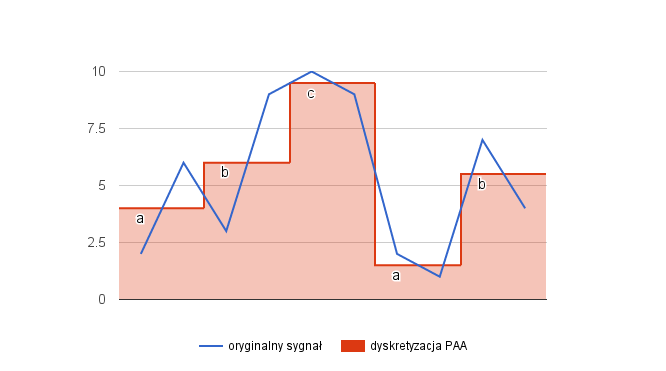
\includegraphics[width=15cm]{figures/sax_moj}

\caption{Oryginalny sygnał z dyskretyzacją i naniesionym SAXem}


\end{figure}
co oznacza, że ostatecznym wynikiem metody SAX dla szeregu czasowego
$x$ przy zadanych parametrach długości łańcucha wyjściowego 5 oraz
alfabetu trójelementowego jest ciąg znaków $abcab$.


\section{DTW (Dynamic Time Warping)}

Algorytm DTW jest metodą, która stara się wyeliminować błąd porównywania
dwóch szeregów czasowych, których charakterystyczne cechy były wobec
siebie nieco przesunięte w czasie bądź w jednym szeregu zdarzenie
postępowało wolniej niż w drugim - choć nadal było to to samo zdarzenie.
Potrafi też poradzić sobie z pojedynczymi błędami pomiaru czy drobnymi
szumami. Te cechy widać na rysunku \ref{fig:Dopasowywanie-DTW} na
którym sygnał \dcscode{vec1} wyraźnie dostosowuje się do sygnału
\dcscode{vec2} mimo dużego spadku wartości w połowie przebiegu.

\begin{figure}[tbph]
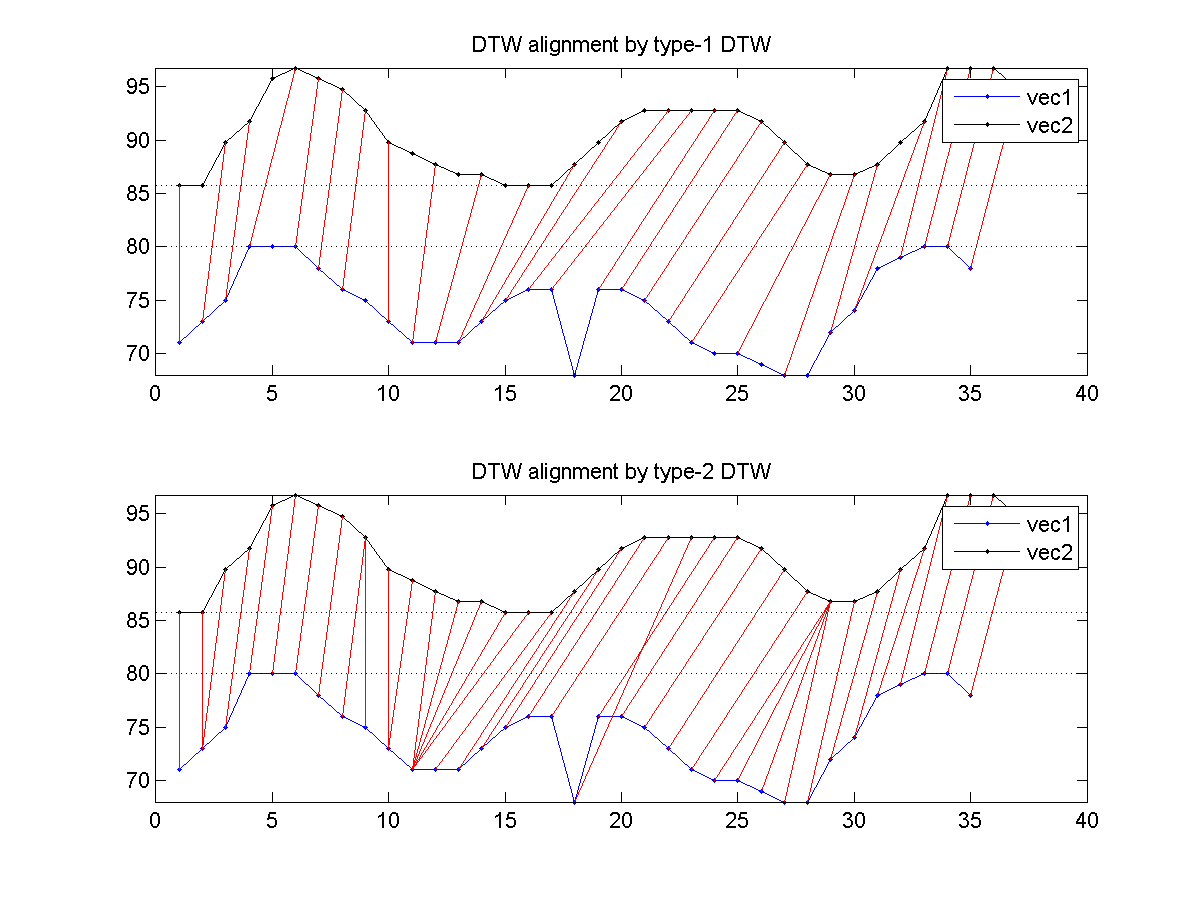
\includegraphics[width=15cm]{other/dtwBridgePlot02}

\caption{Dopasowywanie DTW\cite{chinczyk}\label{fig:Dopasowywanie-DTW}}
\end{figure}


To jak realizowany jest algorytm DTW obrazuje rysunek \ref{fig:Macierz-DTW}.
W momencie przyrównywania dwóch sygnałów, tworzona jest macierz odległości,
której wartości obliczane są rekurencyjnie. Ostatni wiersz macierzy
to różnice między kolejnymi wartościami szeregów. Kolejne wiersze
powstają na ich podstawie. Gdy macierz jest już skonstruowana, wybiera
się najkrótszą kosztowo ścieżkę między skrajnymi wierzchołkami macierzy
- suma wartości komórek, przez które przechodzi ścieżka jest dystansem
między tymi szeregami.
\begin{figure}[tbph]
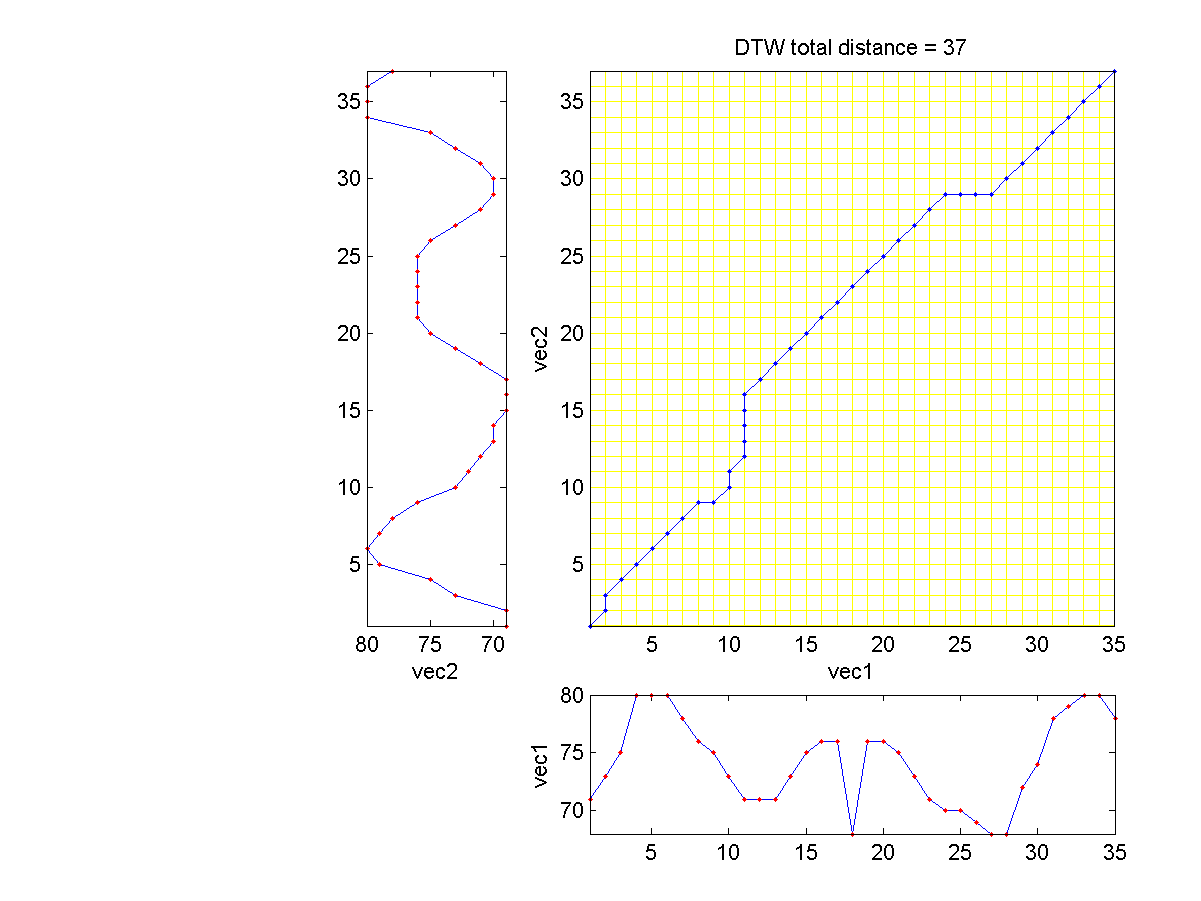
\includegraphics[width=15cm]{other/dtw2Plot01}

\caption{Macierz DTW\cite{chinczyk}\label{fig:Macierz-DTW}}


\end{figure}
 Należy nadmienić, że metoda ta jest dokładna, lecz za jej skutecznością
idzie spory nakład czasowy - czas przetwarzania jest nieporównywalnie
większy od pozostałych metod. Szczegółowo zostanie to omówione w rozdziale
poświęconym wynikom.

Teoretycznie metoda jako parametr przyjmuje szerokość okna DTW - określa
to ramy części macierzy, na której można szukać ścieżki pomiędzy wierzchołkami.
Jednak ze względu na wspomniany już ogromny narzut czasowy, metoda
została odpalona tylko na jednej konfiguracji o najmniejszym możliwym
- dwuelementowym - oknie DTW.


\section{Badane zbiory danych}

Jak wspomniano wcześniej, podstawowy zbiór, który miał zostać zbadany
to pacjenci z jaskrą (lub bez). Z tego powodu będzie on opisany nieco
szerzej niż pozostałe zbiory


\subsection{Pacjenci}

Zbiór dostarczony przez dr. J. Błaszczyńskiego. Zbiór zawiera pomiary
dla 116 pacjentów, z których 65 to pacjenci zdrowi, a 51 to pacjenci
ze zdiagnozowaną jaskrą. Dla każdego pacjenta zebrano 288 pomiarów
(pomiar co 5 minut przez całą dobę) tzw. TFADJ (Trigger Fish Adjusted)
będącym przekształceniem zmierzonego w danym momencie ciśnienia w
oku. Poniżej poglądowe zdjęcie metody zbierania pomiarów:

\begin{figure}[tbph]
\includegraphics[width=15cm]{\string"C:/Users/womi/Documents/prv/TimeSeries/doc/rozne/pomiar jaskry\string".png}

\caption{Metoda zbierania pomiarów od pacjentów}


\end{figure}



\subsection{Dane prof. Eamonna Keogh'a\cite{UCRArchive}}

Zbiory pobrane od prof. Eamonna nie zawierają opisu poszczególnych
zbiorów, dlatego też ich tu nie przedstawiono. Jednak przetwarzając
dane można było wyciągnąć z nich pewne interesujące statystyki, które
przedstawiono w poniższej tabeli (w ostatnim wierszu porównawczo zestawiono
zbiór dr. Błaszczyńskiego):

\begin{table}[tbph]
\caption{Szczegóły danych\label{tab:Szczeg=0000F3=000142y-danych}}


\begin{tabular}{c>{\centering}p{2.5cm}>{\centering}p{1.5cm}>{\raggedright}p{3.5cm}>{\centering}p{1.7cm}}
\hline 
\dcsstrong{nazwa zbioru} & \dcsstrong{liczba instancji} & \dcsstrong{liczba klas} & \dcsstrong{podział na klasy} & \dcsstrong{długość szeregu}\tabularnewline
\hline 
ECG200 & 200

~ & 2 & \multirow{1}{3.5cm}{'-1' - 67 rekordów '1'~-~133~rekordów} & 96\tabularnewline
\hline 
ECGFiveDays & 884 & 2 & '1' - 442 rekordów 

'2' - 442 rekordów & 136\tabularnewline
\hline 
TwoLeadECG & 1162 & 2 & '2' - 581 rekordów 

'1' - 581 rekordów & 82\tabularnewline
\hline 
Yoga & 3300 & 2 & '1' - 1530 rekordów 

'2' - 1770 rekordów & 426\tabularnewline
\hline 
MoteStrain & 1272 & 2 & '2' - 587 rekordów

'1' - 685 rekordów & 84\tabularnewline
\hline 
ItalyPowerDemand & 1096 & 2 & '1' - 547 rekordów 

'2' - 549 rekordów & 24\tabularnewline
\hline 
ChlorineConcentration & 4307 & 3 & '1' - 1000 rekordów 

'3' - 2307 rekordów 

'2' - 1000 rekordów & 166\tabularnewline
\hline 
Two Patterns & 5000 & 3 & '2' - 1248 rekordów 

'3' - 1245 rekordów 

'4' - 1201 rekordów 

'1' - 1306 rekordów & 128\tabularnewline
\hline 
Wafer & 7174 & 2 & '1' - 6402 rekordów

'-1' - 762 rekordów & 152\tabularnewline
\hline 
InlineSkate & 650 & 7 & '2' - 100 rekordów 

'3' - 103 rekordów 

'7' - 62 rekordów 

'6' - 98 rekordów 

'4' - 108 rekordów 

'5' - 117 rekordów 

'1' - 62 rekordów & 1882\tabularnewline
\hline 
\dcsemph{Pacjenci } & \dcsemph{116} & \dcsemph{2} & \dcsemph{'0' - 65 rekordów \\
'1' - 51 rekordów} & \dcsemph{288}\tabularnewline
\hline 
\end{tabular}
\end{table}



\chapter{Koncepcja projektu}


\section{Metody przetwarzania danych dla klasyfikatorów}

W celu osiągnięcia jak najlepszych wyników, postanowiono przy rozpoczęciu
prac nad tą pracą dyplomową spróbować podejścia polegającego na zmodyfikowaniu
sygnału wejściowego przed przekazaniem go do klasyfikatora. Zrealizowano
to na kilka sposobów, które zostały opisane w niniejszym podrozdziale.


\subsection{Dzielenie sygnału na części}

Pierwszym oraz jeden z prostszych koncepcyjnie pomysłów jaki został
wdrożony było podzielenie wejściowego sygnału na części. Przykładowo
dla regresji znacznie dzięki temu wzrasta liczba atrybutów, a co za
tym idzie - dokładność klasyfikacji. Tak jak klasyczna regresja zwróci
dwa argumenty - parametr \dcscode{a} oraz \dcscode{b}, tak po podzieleniu
sygnału na 3 części dostaniemy aż trzy pary takich parametrów. Jako
możliwe wartości tego parametru na przestrzeni eksperymentów wybrano
1, 3 oraz 5. Dodatkowo dla eksperymentu z regresją dodano dodatkowe
10, 20 oraz 48.


\subsection{Podejście SAX}

Opisana wyżej metoda dyskretyzacji sygnału została użyta do kilku
spośród przeprowadzonych eksperymentów. Żeby zbadać różne możliwości
przebiegu tej dyskretyzacji zdecydowano się na parametryzację tej
metody. W ramach dopuszczalnych długości alfabetu wybrano 3, 5 oraz
11 znaków, a w kwestii długości łańcucha wynikowego zdecydowano się
na stałą długość 96 znaków.


\subsection{Zliczanie (eksperyment ,,Counted'')}

Metoda zliczania ściśle bazuje na metodzie SAX - modyfikacje danych
następują na poziomie wynikowego łańcucha znaków, a nie czystego szeregu
czasowego. Pierwszym krokiem zatem jest wyliczenie łańcucha SAX dla
instancji. Następnie łańcuch ten dzieli się na zadaną liczbę części.
W kolejnym kroku potrzebny jest kolejny parametr - ngram - który może
przyjąć wartość 2 lub 3. Polega on na zliczeniu wszystkich możliwych
2- lub 3gramów w łańcuchu badanej części. Wynikiem są wystąpienia
danych ngramów w każdej z części. Poniżej przedstawiono to na przykładzie.

Dla tego przykładu przyjęto podane założenia: metoda otrzymuje 3 rekordy,
a dla ich sygnałów metoda SAX wyliczyła odpowiednie łańcuchy:
\begin{itemize}
\item r1: 'abaabbbbaabb' z przypisaniem do klasy '1'
\item r2: 'abbabaaaabba' z przypisaniem do klasy '1'
\item r3: 'aaababbbaaaa' z przypisaniem do klasy '2'
\end{itemize}
W tabeli zamieszczono przebieg algorytmu dla podziału na 3 części
oraz wyszczególniono 2gramy pojawiające się w ramach każdej z części.

\begin{table}[tbph]
\begin{tabular}{|c|c|c|c|}
\hline 
 & okres 1 & okres 2 & okres 3\tabularnewline
\hline 
\hline 
\textbf{rekord 1} & \textbf{abaa} & \textbf{bbbb} & \textbf{aabb}\tabularnewline
\hline 
 & ab & bb & aa\tabularnewline
\hline 
 & ba &  & ab\tabularnewline
\hline 
 & aa &  & bb\tabularnewline
\hline 
\hline 
\textbf{rekord 2} & \textbf{abba} & \textbf{baaa} & \textbf{abba}\tabularnewline
\hline 
 & ab & ba & ab\tabularnewline
\hline 
 & bb & aa & bb\tabularnewline
\hline 
 & ba &  & ba\tabularnewline
\hline 
\hline 
\textbf{rekord 3} & \textbf{aaab} & \textbf{abbb} & \textbf{aaaa}\tabularnewline
\hline 
 & aa & ab & aa\tabularnewline
\hline 
 & ab & bb & \tabularnewline
\hline 
\end{tabular}

\caption{Podział łańcuchów SAX instancji na 2gramy 'Counted'\label{tab:Podzia=000142-=000142a=000144cuch=0000F3w-SAX}}


\end{table}
W kolejnym kroku należy zliczyć ile razy wystąpił każdy z 2gramów.
Wyniki przedstawia tabela 

\begin{table}[tbph]
\begin{tabular}{|c|c|c|c|}
\hline 
 & rekord 1 & rekord 2 & rekord 3\tabularnewline
\hline 
\hline 
o1ab & 1 & 1 & 1\tabularnewline
\hline 
o1ba & 1 & 1 & 0\tabularnewline
\hline 
o1aa & 1 & 0 & 2\tabularnewline
\hline 
o1bb & 0 & 1 & 0\tabularnewline
\hline 
\hline 
o2bb & 3 & 0 & 2\tabularnewline
\hline 
o2ba & 0 & 1 & 0\tabularnewline
\hline 
o2aa & 0 & 2 & 0\tabularnewline
\hline 
o2ab & 0 & 0 & 1\tabularnewline
\hline 
\hline 
o3aa & 1 & 0 & 3\tabularnewline
\hline 
o3ab & 1 & 1 & 0\tabularnewline
\hline 
o3bb & 1 & 1 & 0\tabularnewline
\hline 
o3ba & 0 & 1 & 0\tabularnewline
\hline 
\end{tabular}

\caption{Zliczenie 2gramów dla instancji przedstawionych w \ref{tab:Podzia=000142-=000142a=000144cuch=0000F3w-SAX}
\label{tab:Zliczenie-2gram=0000F3w} }
\end{table}
Na podstawie tabeli \ref{tab:Zliczenie-2gram=0000F3w} generowany
jest plik wejściowy \dcscode{arff}dla klasyfikatora, który dla omawianego
przykładu wyglądałby tak, jak pokazano w listingu \ref{code:Wynikowy-plik-arff-counted}.
\inputencoding{latin2}\begin{lstlisting}[caption={Wynikowy plik arff dla eksperymentu 'Counted'},label={code:Wynikowy-plik-arff-counted}]
@relation 'Sax counted'

@attribute o1ab numeric
@attribute o1ba numeric
@attribute o1aa numeric
@attribute o1bb numeric
@attribute o2bb numeric
@attribute o2ba numeric
@attribute o2aa numeric
@attribute o2ab numeric
@attribute o3aa numeric
@attribute o3ab numeric
@attribute o3bb numeric
@attribute o3ba numeric

@attribute destClass {1,2}

@data
1,1,1,0,3,0,0,0,1,1,1,0,1
1,1,0,1,0,1,2,0,0,1,1,1,1
1,0,2,0,2,0,0,1,3,0,0,0,2
\end{lstlisting}
\inputencoding{utf8}


\subsection{Dominacja (eksperyment ,,Dominant'')}

Eksperyment nazwany eksperymentem dominacyjnym jest łudząco podobny
do eksperymentu 'Counted' - różni się jedynie sposobem zliczania ngramów,
dlatego zostanie zobrazowany na tym samym przykładzie. Tym razem analizując
każdy z ngramów w poszczególnej części zlicza się ngramy będące co
najmniej tak samo ,,wysokie'' na każdym z argumentów (tutaj: znaków
w łańcuchu) w opcji 'atMost' lub też co najwyżej tak samo opisany
na każdym z argumentów ('atLeast') jak ten badany. W tabeli \ref{tab:Dominacja-ngram=0000F3w}
przedstawiono jak wyglądają wyniki zliczania z dominacją dla rekordów
przedstawionych w tabeli \ref{tab:Podzia=000142-=000142a=000144cuch=0000F3w-SAX}. 

\begin{table}[tbph]
\begin{tabular}{|c|c|c|c|}
\hline 
 & rekord 1 & rekord 2 & rekord 3\tabularnewline
\hline 
\hline 
o1<=ab & 2 & 1 & 3\tabularnewline
\hline 
o1>=ab & 1 & 2 & 1\tabularnewline
\hline 
o1<=bb & 3 & 3 & 3\tabularnewline
\hline 
o1>=bb & 0 & 1 & 0\tabularnewline
\hline 
o1<=ba & 2 & 1 & 2\tabularnewline
\hline 
o1>=ba & 1 & 2 & 0\tabularnewline
\hline 
o1<=aa & 1 & 0 & 2\tabularnewline
\hline 
o1>=aa & 3 & 3 & 3\tabularnewline
\hline 
\end{tabular}

\caption{Dominacja ngramów dla rekordów z tabeli \ref{tab:Podzia=000142-=000142a=000144cuch=0000F3w-SAX}\label{tab:Dominacja-ngram=0000F3w}}


\end{table}
 

Jak można zauważyć, w takim podejściu podwaja się liczba argumentów
dla każdego rekordu (w tabeli przestawiono tylko część dotyczącą pierwszego
okresu - stąd prefiksy 'o1'). Wartość '2' dla rekordu 1 w wierszu
o1<=ab oznacza, że spośród ngramów w tym okresie dwa z nich były co
najwyżej takie jak 2gram 'ab' - są to 2gramy 'ab' oraz 'aa' - oba
występowały jednokrotnie. Z kolei na przykład wartość 0 dla rekordu
3 w wierszu o1>=ba oznajmia, że nie było żadnego 2gramu większego
lub równego 2gramowi 'ba' w łańcuchu odzwierciedlającym przebieg sygnału
dla rekordu nr 3.

Jak zauważono, dla ngramów prezentujących co najmniej najmniejsze
lub co najwyżej największe wartości na każdym ze znaków łańcucha,
wartości zliczeń są zawsze maksymalne (w tym przykładzie wiersze 'o1<=bb'
oraz 'o1>=aa'). Nie wnoszą zatem one żadnej informacji godnej uwagi
klasyfikatora, zatem wiersze te były wycinane przed eksportem do pliku
arff.

Ze względów technicznych w plikach arff znaki '<=', '>=' zostały zmienione
na 'atL', 'atM' czyli odpowiednio atLeast (co najmniej) oraz at Most
(co najwyżej). W listingu \ref{code:Wynikowy-plik-arff-dominant}
przedstawiono pełny plik arff dla omawianego przypadku w wariancie
eksperymentu 'Dominant'. \inputencoding{latin2}
\begin{lstlisting}[caption={Wynikowy plik arff dla eksperymentu 'Dominant'},label={code:Wynikowy-plik-arff-dominant}]
@relation 'Sax dominant'

@attribute o1atMaa numeric
@attribute o1atMab numeric
@attribute o1atLab numeric
@attribute o1atMba numeric
@attribute o1atLba numeric
@attribute o1atLbb numeric
@attribute o2atLbb numeric
@attribute o2atMaa numeric
@attribute o2atMba numeric
@attribute o2atLba numeric
@attribute o2atMab numeric
@attribute o2atLab numeric
@attribute o3atMaa numeric
@attribute o3atLbb numeric
@attribute o3atMab numeric
@attribute o3atLab numeric
@attribute o3atMba numeric
@attribute o3atLba numeric
@attribute destClass {1,2}

@data
1,2,1,2,1,0,3,0,0,3,0,3,1,1,2,2,1,1,1
0,1,2,1,2,1,0,2,3,1,2,0,0,1,1,2,1,2,1
2,3,1,2,0,0,2,0,0,2,1,3,3,0,3,0,3,0,2
\end{lstlisting}
\inputencoding{utf8}


\subsection{K najbliższych sąsiadów (ang. KNN - k Nearest Neighbors)}

W eksperymencie zorientowanym wokół algorytmu KNN zdecydowano się
na dość nowatorskie podejście z dyskretyzacją danych. Przeważnie używając
algorytmu najbliższych sąsiadów, za dane wejściowe uznaje się czysty
zebrany sygnał. W tym projekcie postanowiono zdyskretyzować dane używając
do tego metody SAX, a dopiero potem przekazać jej rezultat do klasyfikatora
KNN, dzięki czemu zyskaliśmy swego rodzaju normalizację danych.


\subsection{Bagging}

Przygotowanie danych dla eksperymentu Bagging przebiegało dokładnie
w ten sam sposób co dla eksperymentu Zliczającego. Eksperymenty różniły
się sposobem użycia klasyfikatora. Oba eksperymenty skorzystały z
\dcscode{J48}, lecz dla Baggingu był on opakowany w meta-klasyfikator
\dcscode{weka.classifiers.meta.Bagging}, który bliżej zostanie opisany
w podrozdziale \eqref{sub:Bagging}.


\section{Użyte klasyfikatory}


\subsection{J48}

J48 to jeden z podstawowych klasyfikatorów pakietu \dcscode{weka},
opierający algorytm klasyfikacji na drzewach decyzyjnych. Jego działanie
rozpoczyna się na przypisaniu wszystkich instancji treningowych do
jednego liścia. Jeżeli wszystkie elementy należą do tej samej klasy,
to algorytm się kończy - jeśli nie, wybiera atrybut, który najlepiej
rozdziela instancje w liściu na różne klasy i tworzy odpowiedni liść.
Algorytm trwa aż w liściach pozostaną jednorodne grupy elementów lub
nie będzie można dobrać kolejnych atrybutów jako kryterium podziału.


\subsection{IBk}

Klasyfikator stworzony do przeprowadzania klasyfikacji za pomocą algorytmu
k-najbliższych sąsiadów (ang. KNN: K-Nearest-Neighbors) z pakietu
\dcscode{weka}. Dzięki temu, że klasyfikator ten można w łatwy sposób
zmodyfikować na poziomie kodu, dostosowano go również do eksperymentu
DTW, który również bazuje na metodzie KNN, jednak używa innego algorytmu
wyszukiwania ów najbliższych sąsiadów.


\subsection{VC-DomLEM\cite{VcDomLem}}

Algorytm VC-DomLEM bazuje na schemacie sekwencyjnego pokrywania \cite{Michalski1969}\cite{Furnkranz}.
Algorytm ten pokrywa obszary pozytywne, utworzone przez VC-DRSA \cite{BlaszczynskiEtAl},
za pomocą reguł decyzyjnych o wymaganej spójności. VC-DomLEM jest
inspirowany algorytmem LEM2 \cite{Grzymala}, a także adaptacją tego
algorytmu dla danych porządkowych DomLEM \cite{GrecoEtAl}. 


\subsection{Basic Ngram Classifier}

Autorski klasyfikator zbudowany na wzór klasyfikatora pakietu weka
(rozszerza klasę \dcscode{weka.classifiers.Classifier}). Jako wejście
przyjmuje jeden argument - łańcuch wyjściowy z algorytmu SAX. Następnie
dla każdej klasy decyzyjnej wyznacza liczności występowań danych n-gramów
(gdzie n jest parametrem metody). W momencie klasyfikacji instancji
zlicza się występowanie ngramów w ramach badanej instancji, by potem
zmierzyć dystanse dzielące instancję oraz wszystkie klasy decyzyjne.
Instancja zostaje przypisana do klasy, z którą dzieli ją najmniejszy
dystans. Aby przedstawić sposób liczenia tej odległości zdefiniowano
następującą funkcję: $occ(klasa,ngram)$ która jako wynik zwraca ile
wystąpień danego ngramu miało miejsce w ramach podanej klasy decyzyjnej.
Analogicznie $occ(instancja,ngram)$ podaje liczbę wystąpień ngramu
dla zadanej instancji. 

Zatem dla każdej klasy liczony jest następująca odległość między instancją
a klasą:
\[
dist(instance,class)=\sqrt{\sum_{ngram}^{instance}(occ(klasa,ngram)-occ(instancja,ngram))^{2}}
\]



\subsection{Bagging\label{sub:Bagging}}

Bagging\cite{Bagging} to metoda polegająca na generowaniu wielu wersji
klasyfikatora po to by uzyskać kształt klasyfikatora zagregowanego.
Wówczas o przyporządkowaniu instancji do klasy decyduje głosowanie
poszczególnych klasyfikatorów. Kolejne wersje klasyfikatora powstają
na podstawie wylosowanej (losowanie ze zwracaniem) próby instacji
na której wybrany klasyfikator przeprowadza uczenie.


\section{Miary\cite{ActivityLearning}}

Do oceniania poprawności eksperymentów wybrano sześć miar statystycznych.
Niektóre z nich bazują na kilku definicjach c \dcsemph{confussion matrix},
których znaczenie przedstawiono w tabeli poniżej:

\begin{tabular}{|>{\centering}p{4cm}|>{\centering}m{4cm}|>{\centering}m{4cm}|}
\cline{2-3} 
\multicolumn{1}{>{\centering}p{4cm}|}{} & Rzeczywista wartość pozytywna & Rzeczywista wartość negatywna\tabularnewline
\hline 
Przewidywana wartość pozytywna & \textbf{True Positive} & \textbf{False Positive}\tabularnewline
\hline 
Przewidywana wartość negatywna & \textbf{False Negative} & \textbf{True Negative}\tabularnewline
\hline 
\end{tabular}


\subsection{Dokładność (ang. accuracy)}

Najbardziej znana i intuicyjna miara ewaluacji klasyfikatora to właśnie
dokładność. Określa ją stosunek poprawnie sklasyfikowanych instancji
do liczby wszystkich instancji. Dzięki swojej prostej koncepcji może
być z powodzeniem używana zarówno w problemach binarnych jak i wieloklasowych.
\[
Accuracy=\frac{correctly\,classified\,instances}{total\,instances}
\]



\subsection{Wrażliwość (ang. sensitivity)}

Miara ta, znana również pod nazwą \dcsemph{True positive rate}, skupia
się na zobrazowaniu stosunku instancji poprawnie zidentyfikowanych
w klasie umownie uznanej za pozytywną do liczby instancji w tej klasie.
Na przykładzie zbioru Pacjentów opisywanego w tej pracy można powiedzieć,
że jest to proporcja pacjentów poprawnie sklasyfikowanych jako chorzy
na jaskrę do wszystkich, którzy są na tę jaskrę chorzy. Wzór na wrażliwość
podano poniżej:
\[
Sensitivity=\frac{TP}{TP+FN}
\]



\subsection{Specyficzność (ang. specificity)}

Specyficzność to w pewnym sensie przeciwieństwo wrażliwości - uwydatnia
proporcję instancji dobrze sklasyfikowanych w klasie uznanej umownie
za negatywną do liczby instancji w tej klasie. Ponownie odwołując
się do analizowanych tutaj Pacjentów wynik specyficzności to iloraz
pacjentów prawidłowo sklasyfikowanych jako zdrowi i liczby wszystkich
zdrowych pacjentów. Poniżej przedstawiono jej wzór ogólny:
\[
Specificity=\frac{TN}{TN+FP}
\]



\subsection{Średnia geometryczna (ang. geometric mean)}

Miara \dcsemph{G-mean} to geometryczne uśrednienie miar wspomnianych
powyżej, czyli wrażliwości i specyficzności. Estymuje więc skuteczność
klasyfikatora zarówno na klasie pozytywnej jak i negatywnej. Dla formalności
poniżej przedstawiono jej wzór:
\[
Gmean=\sqrt{\frac{TP}{TP+FN}\times\frac{TN}{TN+FP}}=\sqrt{Sensitivity\times Specificity}
\]
Jak można zauważyć dalej w wynikach, dla zbiorów wieloklasowych miary
Sensitivity, Specificity oraz GMean nie były obliczane, ze względu
na to, że musiałyby zostać przedstawione dla każdej klasy osobno.
Porównywanie takich wyników między zbiorem trójklasowym a siedmioklasowym
byłoby niemiarodajne, dlatego też w zbiorach posiadających co najmniej
3 klasy zrezygnowano z obliczania tych trzech miar.


\subsubsection{Miara F (ang. F-measure, F1)}

Na potrzeby zobrazowania miary F posłużono się definicjami precyzji
(ang. precision) oraz przywołania (ang. recall). Precyzja wyraża to
ile było trafień w klasie pozytywnej w odniesieniu do wszystkich instancji,
które klasyfikator uznał za należące do klasy pozytywnej ($Precision=\frac{TP}{TP+FP})$.
Przywołanie natomiast to nic innego co wspomniana już wcześniej wrażliwość.
Miara F1 zaś jest dwukrotnym ilorazem iloczynu precyzji i przywołania
oraz ich sumy: 
\[
F1=2\frac{precision\times recall}{precision+recall}
\]



\subsection{Procent poprawnie sklasyfikowanych (ang. Percent Correctly Classified)}

Jest to prosta miara uwidaczniająca udział prawidłowo sklasyfikowanych
instancji w odniesieniu do ogółu. Jej wzór prezentuje się następująco:
\[
PCC=\frac{correctly\,classified\,instances}{instances}
\]



\section{Posumowanie}

Jak szczegółowo opisano wyżej, przeprowadzono aż 7 zróżnicowanych
eksperymentów na 11 zbiorach danych. W tabeli \ref{tab:Lista-eksperyment=0000F3w}
przedstawiono zebrane informacje dotyczące tego jak przetworzono dane
zanim przekazano je do klasyfikatora oraz jaki klasyfikator te dane
przeliczał. Dla przejrzystości użyto skrótu 'sax' dla pary parametrów:
rozmiar ngramu oraz liczba liter w alfabecie.

\begin{table}[tbph]
\begin{tabular}{|>{\centering}p{3cm}|>{\centering}p{6cm}|>{\centering}p{3cm}|>{\centering}p{3cm}|}
\hline 
\textbf{Nazwa eksperymentu} & \textbf{dane wejściowe} & \textbf{klasyfikator} & \textbf{parametry}\tabularnewline
\hline 
Regresja & oryginalny sygnał & J48 & części\tabularnewline
\hline 
Dominacja & zliczone dominujące n-gramy SAX & VC-DomLEM & części, sax\tabularnewline
\hline 
Zliczanie & zliczone n-gramy SAX & J48 & części, sax\tabularnewline
\hline 
Ngram & SAX & NgramClassifier & sax\tabularnewline
\hline 
KNN & sygnał zdyskretyzowany metodą SAX & IBk & sax, k\tabularnewline
\hline 
DTW & oryginalny sygnał & IBk & k, okno dtw\tabularnewline
\hline 
Bagging & zliczone n-gramy SAX & J48 & części, sax\tabularnewline
\hline 
\end{tabular}

\caption{Zrealizowane eksperymenty\label{tab:Lista-eksperyment=0000F3w}}
\end{table}



\chapter{Implementacja}


\section{Koncepcja budowy biblioteki}

Wiodącym założeniem przyświecającym pracom implementacyjnym nad biblioteką
obliczeniową było podążanie za dobrymi praktykami wytwarzania oprogramowania
według Roberta C. Martina - z głównym naciskiem na OCP (Open Closed
Principle)\cite{MartinPrinciples} - zasadę ,,otwarte-zamknięte''.
Oznacza to, że oprogramowanie ma być otwarte na zmiany, lecz zamknięte
na modyfikacje - starano się zatem osiągnąć stan, w którym istniejący
kod można rozszerzyć z jak najmniejszym wysiłkiem wniesionym w edycję
istniejącego kodu. Szczegóły tej idei przedstawiono w poniższych sekcjach.


\subsection{Użyte biblioteki pomocnicze}

Żeby móc w pełni opisać funkcjonalność i sposób budowy programu należy
nadmienić jakimi bibliotekami wspomagano się podczas tego procesu.


\subsubsection{Weka}

Najważniejsza biblioteka, z którą program współpracuje najściślej.
Wiedząc, że Weka jest często używana do klasyfikacji czy uczenia maszynowego,
autor chciał stworzyć narzędzie kompatybilne z programem stworzonym
na Uniwersytecie w australijskim Waikato. Kilka kluczowych klas programu
autora rozszerza klasy pakietu \dcscode{weka} stwarzając możliwości
wykorzystania rozmaitych składowych tego systemu. Ponadto używanie
klas takich jak \dcscode{weka.classifiers.Evaluation} do przeprowadzania
eksperymentów daje pewność, że wykorzystywane rozwiązanie jest dobrze
przetestowane i powinno zwracać rzetelne wyniki. Stąd również przyjęto
format wyjściowy plików klasyfikacyjnych \dcscode{{*}.arff}


\subsubsection{jMotif}

Z pakietu \dcscode{jMotif} zaczerpnięto metody zajmujące się tworzeniem
łańcucha danych na podstawie zadanego szeregu czasowego za pomocą\ algorytmu
SAX.


\subsubsection{JFreeChart}

Biblioteka służąca do rysowania wykresów. Bardzo pomocna w początkowej
fazie implementacji, kiedy autorowi zależało na zobrazowaniu przebiegu
szeregów czasowych. Ich wizualizacja mogła przyczynić się do lepszego
zrozumienia zależności między przebiegami, a diagnozą pacjenta.


\subsubsection{Jxl}

Dzięki pakietowi \dcscode{jxl}w początkowej fazie implementacji autor
mógł ściśle współpracować z arkuszami kalkulacyjnymi w celu raportowania
danych do plików .xls w celu ich dalszej analizy statystycznej.


\subsubsection{joda-time}

W momencie gdy prace nad tą pracą dyplomową zostały rozpoczęte, wsparcie
dla obiektów typu data czy czas było dla autora niewystarczające,
dlatego zdecydowano się na wykorzystanie biblioteki \dcscode{joda-time}
w celu zapewnienia wymaganej obsługi tego rodzaju danych.


\subsubsection{fast-dtw}

Pakiet fast-dtw dostarcza obsługę obliczeniową dla eksperymentu bazującego
na algorytmie Dynamic Time Warping, dzięki czemu autor mógł skorzystać
z gotowego, przetestowanego i relatywnie wydajnego czasowo i pamięciowo
rozwiązania dla tego celu.


\subsubsection{apache-commons}

W momentach gdy brakowało pewnych struktur danych w obecnej wersji
Java - takich jak choćby Pair (ang. para) lub należało skorzystać
z popularnych metod takich jak obliczenie regresji, korzystano z bibliotek
apache-commons.


\subsection{Punkt wyjścia}

Praca programu zorientowana jest wokół obiektu \dcscode{Workflow}
(ang. ,,przepływ'', ,,proces'') - ma on na celu zdefiniowanie
następujących po sobie kroków składających się na przebieg eksperymentu
- począwszy od wczytania danych, aż do wypisania ostatecznego wyniku.
Jego rdzeń zawiera się w abstrakcyjnej klasie \dcscode{WorkflowBase}
która posiada trzy główne metody - odpalenia przebiegu pełnego eksperymentu,
wygenerowania pliku arff dla eksperymentu oraz wyliczenia wyniku eksperymentu
dla zadanego pliku arff. Ponadto jest w stanie opisać podstawowe statystyki
wczytanych danych, takie jak liczba klas decyzyjnych, podział instancji
w klasach, czy liczba atrybutów w ramach instancji. Aby stworzyć własny
eksperyment wystarczy stworzyć klasę dziedziczącą z \dcscode{WorkflowBase}
oraz zaimplementować wymagane metody. Przykładowy szkic takiej klasy
przedstawiono na listingu \ref{code:Kod-eksperymentu-Counted}:\inputencoding{latin2}
\begin{lstlisting}[caption={Kod eksperymentu Counted},label={code:Kod-eksperymentu-Counted},language=Java,float,numbers=left,tabsize=4]
public class CountedWorkflow extends WorkflowBase {

	private List<CalculatedRecord> calculatedRecords;

	public CountedWorkflow(DivisionOptions divisionOption, boolean glaucoma) {
		super(divisionOption, glaucoma);
	}

	@Override
	protected Instances buildInstances() {
		exporter = new CountedSaxArffBuilder(calculatedRecords);
		return exporter.buildInstances();
	}

	@Override
	protected void processData() throws Exception {
		calculatedRecords = new ArrayList<CalculatedRecord>();

		for (IRecord record : records) {
			ArrayList<HashMap<String, Integer>> periodicallyCountedNgrams = 
									new ArrayList<HashMap<String, Integer>>();

			List<String> dividedSax = DataDivider.divideStringRegularly(
					record.getSaxString(), divisionPartsAmount);

			for (String elem : dividedSax) {
				HashMap<String, Integer> ngramCountMap = PeriodicNgramCounter
						.slashStringAndCountNgrams(elem, windowLen);
				periodicallyCountedNgrams.add(ngramCountMap);
			}

			CalculatedRecord calcRecord = new CalculatedRecord(
					periodicallyCountedNgrams, record.getDestinationClass());
			calculatedRecords.add(calcRecord);
		}
	}

	@Override
	protected void setConcerningParams() {
		concerningParameters.add(Pair.of("parts", divisionPartsAmount));
		concerningParameters.add(Pair.of("ngram", windowLen));
		concerningParameters.add(Pair.of("alpha", Config.getInstance().getSaxAlphabeatSize()));
	}
}
\end{lstlisting}
\inputencoding{utf8}Jeżeli wczytane przez nas dane wymagają jakiejkolwiek ingerencji obliczeniowej
- tak jak na przykład eksperyment Counted, to fragment kodu odpowiadający
za te obliczenia powinien znaleźć się w metodzie \dcscode{processData}.
Jak widać w przywołanym listingu, wszystkie wymagane obliczenia odbywają
się w tym fragmencie kodu. Kolejna metoda to \dcscode{buildInstances}
która odpowiada za ustawienie odpowiedniego eksportera danych (w szczegółach
zostanie omówiony niżej) oraz przekazanie mu przeliczonych danych.
Za jego pomocą tworzony jest obiekt \dcscode{Instaces}, który musi
zostać zwrócony jako wynik metody. Funkcja \dcscode{setConcerningParams}służy
już tylko do tego, aby podczas wyświetlania wyniku eksperymentu wypisać,
które parametry programu mają wpływ na pracę tego eksperymentu, oraz
jakie ich wartości zostały ustawione podczas bieżącego wykonania. 


\subsection{Importowanie danych}

Importowanie danych zostało rozdzielone ze względu na dwa różne formaty
danych jakie potrafi wczytać program. Ostateczną wersją danych pacjentów
jest opisanie danych każdego pacjenta w osobnym pliku \dcscode{.csv}.
W każdym z nich podany jest identyfikator pacjenta, oraz dane z poszczególnych
pomiarów ciśnienia w oku. W ramach każdego pomiaru udostępnionych
jest sporo danych, takich jak godzina o której pomiar został zdjęty,
pozycja ciała w której znajdował się pacjent itp. choć na potrzebę
tej pracy korzystano tylko z miary \dcscode{TFADJ}. Jedyna informacja,
której nie ma w tym pliku to diagnoza - ta opisana jest w pliku zbiorczym
dla wszystkich pacjentów. W kolejnych wierszach znajdują się pary
identyfikator pacjenta - diagnoza.

Drugim formatem, jaki wspiera program jest format danych prof. Eamonna.
Ich charakterystyka jest prosta - każdy nowy wiersz w pliku to nowa
instancja. W ramach każdego wiersza figurują atrybuty oddzielone spacjami,
z których pierwszy to atrybut decyzyjny, a kolejne to szereg wartości
składające się w szereg czasowy dla tej instancji. Tak jak wspomniano
wcześniej, zapis ten pomija dokładny czas zebrania pomiaru. Klasy
odpowiadające za wczytywanie danych to odpowiednio \dcscode{PatientDataImporter2}
oraz \dcscode{DataImporterEamonn}.


\subsection{Eksportowanie pliku arff}

Jedną z funkcji programu jest wygenerowanie pliku \dcscode{arff}
w którym zapisane są już przetworzone dane o instancjach, gotowe do
klasyfikacji klasyfikatorami \dcscode{weki}. Aby stworzyć taki eksporter
na własny użytek można posiłkować się klasą abstrakcyjną \dcscode{ArffExporterBase}
i rozszerzyć ją. Eksporter taki zostanie poniżej opisany na przykładzie
\dcscode{RegressionArffBuilder}. Jego kod można znaleźć na listingu
\ref{code:RegressionExporter}. Klasa nadrzędna wymaga od programisty
zaimplementowania dwóch metod oraz konstruktora. 

Metoda \dcscode{setAttributes} służy do tego aby nadać i nazwać atrybuty
dla formatu danych jaki zdecydowano użyć w docelowym pliku \dcscode{arff}.
W pliku dla eksperymentu Regression tworzy się tyle par \dcscode{slope-intercept}
(współczynników a i b regresji) na ile części został podzielony sygnał.
Należy również pamiętać o tym aby w liście atrybutów zawrzeć również
atrybut decyzyjny.

W funkcji buildInstances programista musi obsłużyć przeniesienie danych
ze struktury w jakiej trzymał dane po ewentualnych obliczeniach w
metodzie \dcscode{processData} klasy \dcscode{WorkflowBase} do obiektu
\dcscode{Instances}. Dzięki temu umożliwione będzie wygodne eksportowanie
pliku \dcscode{arff} oraz przeprowadzanie eksperymentu za pomocą
klasy \dcscode{Evaluation}. Ostatnią rzeczą o którą trzeba zadbać,
to wywołanie metod \dcscode{setDestinationClasses} oraz \dcscode{setAttributes}
w konstruktorze tak jak pokazano na wspomnianym listingu.

\inputencoding{latin2}\begin{lstlisting}[caption={Kod eksportera dla eksperymentu Regression},label={code:RegressionExporter},language=Java,numbers=left,tabsize=4]
public class RegressionArffBuilder extends ArffExporterBase {

	private List<RegressionRow> input;

	public RegressionArffBuilder(List<RegressionRow> input) {
		this.input = input;
		setDestinationClasses(input);
		setAttributes();
	}

	protected void setAttributes() {
		attrInfo = new FastVector();

		int regressionCount = input.stream().findFirst().get()
				.getRegressionResults().size();

		for (int i = 0; i < regressionCount; i++) {
			attrInfo.addElement(new Attribute(String.format("slope%d", i + 1)));
			attrInfo.addElement(new Attribute(String.format("intercept%d",
					i + 1)));
		}

		Attribute destClassAttribute = null;
		try {
			destClassAttribute = constructDestinationClassesNominalAttribute(destClasses);
		} catch (Exception e) {
			e.printStackTrace();
		}
		attrInfo.addElement(destClassAttribute);
	}

	@Override
	public Instances buildInstances() {
		instances = new Instances("Regression", attrInfo, input.size());
		instances.setClassIndex(instances.numAttributes() - 1);

		for (RegressionRow row : input) {
			Instance instance = new Instance(attrInfo.size());
			int attrIdx = 0;
			for (RegressionResult regResult : row.getRegressionResults()) {
				instance.setValue(attrIdx++, regResult.getSlope());
				instance.setValue(attrIdx++, regResult.getIntercept());
			}

			int destClassIndex = getIndexOfDestinationClass(row
					.getDestinationClass());
			instance.setValue(attrIdx, destClassIndex);
			instances.add(instance);
		}
		return instances;
	}
}
\end{lstlisting}
\inputencoding{utf8}


\section{Serwisy zewnętrzne}


\subsection{Git}

Dla zapewnienia jak najwyższej jakości kodu oraz niezawodnego dostępu
do niego, używano systemu kontroli wersji, który był dostarczany przez
oprogramowanie \dcscode{git}. Dzięki darmowym serwisom udostępniającym
swoje serwery na potrzeby wersjonowania źródeł, takim jak \dcscode{gitlab.com}
zapewnione było bezpieczeństwo danych, a także wspólny dostęp do postępów
prac zarówno przez autora, jak i promotora. Na potrzeby obsługi tego
narzędzia użyto oprogramowania \dcscode{SourceTree}, które wyraźnie
ułatwia i przyspiesza pracę z systemem \dcscode{git}.


\subsection{Travis}

Portal \dcscode{travis.com} jest to serwis Continuous Integration
ściśle współpracujący z opisanym wyżej \dcscode{gitlab.com}. Jego
zadaniem jest sprawdzanie każdej kolejnej udostępnionej wersji kodu
na serwerze. W momencie gdy pojawia się jego nowa wersja, Travis kompiluje
świeżo pobrany kod, uruchamia wszystkie zamieszczone w kodzie testy
i ocenia tzw. 'build' pozytywnie lub negatywnie. Dzięki organizacji
pracy z takim serwisem Continuous Integration i pokryciu kluczowych
obliczeniowych metod testami, wyłapano wiele błędów implementacyjnych
we wczesnym ich etapie.


\chapter{Wnioski}


\section{Analiza wyników - część podstawowa}

Gdy nadszedł czas na analizę wyników, dla uproszczenia porównań postanowiono
wybrać najlepsze wyniki dla każdego z eksperymentów, a dopiero wówczas
przeanalizować je bliżej. Aby wyłuskać najskuteczniejsze zestawy parametrów
dla każdego z nich posłużono się prostym zliczeniem zbiorów na których
dany zestaw był najlepszy. Po tym kroku zostały wybrane następujące
uruchomienia:
\begin{itemize}
\item Zliczanie - części: 5, ngram: 2, alfabet: 11
\item Regresja - części: 10
\item Klasyfikator ngramowy - ngram: 30, alfabet: 3
\item DTW - knn: 7, szerokość okna DTW: 5
\item KNN - ngram: 3, alfabet: 11, knn: 3
\item Bagging - części: 5, ngram: 3, alfabet: 5 (na 20\% przykładów)
\end{itemize}
Każdy z nich przeprowadzony został z użyciem pięciokrotnej kroswalidacji
powtórzonej trzy razy.

Ze względu na to, że uśrednianie wyników ze wszystkich zbiorów może
być zgubne, postanowiono choć kilkoma słowami opisać wynik na każdym
z badanych zbiorów.


\subsection*{ECG200}

\begin{figure}[tbph]
\includegraphics{\string"other/aggr ecg200\string".png}

\caption{Dokładność eksperymentów na zbiorze ECG200\label{fig:Dok=000142adno=00015B=000107-aggr ecg200}}


\end{figure}
 Dość mały zbiór z relatywnie krótkim szeregiem do przeanalizowania.
W kwestii dokładności klasyfikacji widać zdecydowaną dominację podejścia
\dcsemph{KNN SAX}, któremu zbiór wyraźnie odpowiadał. Nieco niżej,
na podobnym poziomie dokładności, uplasowały się metody \dcsemph{C4.5 regression}
oraz \dcsemph{DTW raw}. Najgorzej z tymi danymi poradziły sobie warianty
\dcsemph{C4.5 ngrams}, \dcsemph{Basic ngrams} oraz \dcsemph{C4.5 bagging ngrams}.
Zły wynik \dcsemph{Basic ngrams} nie zaskakuje - bo jak się okaże
niebawem na większości zbiorów nie wypadł dobrze, jednak poza tym
widać, że algorytmy zliczeniowe nie byłyby dla takiego zbioru najlepszym
wyborem.


\subsection*{ECGFiveDays}

\begin{figure}[tbph]
\includegraphics{\string"other/aggr ecgfivedays\string".png}

\caption{Dokładność eksperymentów na zbiorze ECGFiveDays}


\end{figure}
 Wydaje się, że dość prosty w klasyfikacji zbiór danych - wszystkie
klasyfikacje za wyjątkiem \dcsemph{Basic ngrams} (choć na tę metodę
patrzono z przymrużeniem oka ze względu na kiepskie wyniki na większości
zbiorów) zanotowały znakomitą dokładność w przyporządkowywaniu instancji
do klas. Co cieszy, to fakt, że znów najlepiej poradził sobie algorytm
\dcsemph{KNN SAX} śrubując wynik aż na 99\% poprawnie sklasyfikowanych
przypadków.


\subsection*{TwoLeadECG}

\begin{figure}[tbph]
\includegraphics{\string"other/aggr Twoleadecg\string".png}

\caption{Dokładność eksperymentów na zbiorze TwoLeadECG}


\end{figure}
 Podobnie jak w powyższym zbiorze danych, w \dcsemph{TwoLeadECG}
wszystkie klasyfikatory za wyjątkiem \dcsemph{Basic ngrams} wypadły
bardzo dobrze, jednak tym razem najlepszym z nich okazał się \dcsemph{DTW raw}
- choć jak wspomniano w części teoretycznej - wyniki z tego podejścia
zestawione są raczej w celach porównawczych, biorąc pod uwagę fakt,
że czas spędzony na przetwarzanie jest nieporównywalnie dłuższy niż
w pozostałych przypadkach. Pomijając zatem ten algorytm, najlepszą
lokatę znów zajmuje \dcsemph{KNN SAX}.


\subsection*{Yoga}

\begin{figure}[tbph]
\includegraphics{\string"other/aggr yoga\string".png}

\caption{Dokładność eksperymentów na zbiorze Yoga}


\end{figure}
 \dcsemph{Yoga} nie jest już tak prostym zbiorem jak jej dwaj poprzednicy.
Zbiór ma 3300 instancji oraz charakteryzuje się długością szeregu
426. Poziom skomplikowania odzwierciedla się na wynikach - tym razem
dokładności klasyfikacji rozpościerają się w przedziale $0.667-0.924$.
Znów najlepszymi wynikami pochwalić się mogą dwa wiodące dotąd klasyfikacje
- czyli odpowiednio \dcsemph{KNN SAX} oraz \dcsemph{DTW raw}. Pozostałe
podejścia (oprócz \dcsemph{Basic ngrams}) odnotowały wynik na bardzo
podobnym poziomie. 


\subsection*{MoteStrain oraz ItalyPowerDemand}

\begin{figure}[tbph]
\includegraphics{\string"other/aggr motestrain\string".png}\caption{Dokładność eksperymentów na zbiorze MoteStrain}


\end{figure}
 
\begin{figure}[tbph]
\includegraphics{\string"other/aggr italypowerdemand\string".png}

\caption{Dokładność eksperymentów na zbiorze ItalyPowerDemand}


\end{figure}
 Dwa podobne pod względem wyników, jak i liczby instancji, zbiory.
Choć długość szeregu wyraźnie różna - odpowiednio 84 i 24. Wszystkie
podejścia wypadły zadowalająco, \dcsemph{Basic ngrams} wyjątkowo
nie odstawał odczuwalnie od pozostałych. Tak jak dotychczas, czołówka
pozostała ta sama - \dcsemph{DTW raw} oraz \dcsemph{KNN SAX}.


\subsection*{ChlorineConcentration}

\begin{figure}[tbph]
\includegraphics{\string"other/aggr clorineconcentration\string".png}

\caption{Dokładność eksperymentów na zbiorze ChlorineConcentration}


\end{figure}
 Pierwszy z wieloklasowych zbiorów i również pierwsza zmiana lidera
- w tym przypadku na tle innych najlepszą dokładność uzyskała regresja
ex aequo z \dcsemph{DTW raw}. Warto odnotować, że w porównaniu do
pozostałych, jest to duży zbiór (4307 instancji), a mimo to, tak prosta
ideowo koncepcja jak regresja okazała się być najlepszym wyborem,
co na pewno jest pewnego rodzaju ciekawostką.


\subsection*{TwoPatterns}

\begin{figure}[tbph]
\includegraphics{\string"other/aggr twopatterns\string".png}

\caption{Dokładność eksperymentów na zbiorze TwoPatterns}


\end{figure}
 Kolejny 'sensacyjny' zbiór - tym razem dlatego, że wariantowi \dcsemph{DTW raw}
udało się uzyskać stuprocentową skuteczność, czym zdeklasował swoich
konkurentów. Podobny wynik (aż 99\%) odnotował \dcsemph{KNN SAX},
nieco gorzej \dcsemph{C4.5 bagging ngrams}, a już wyraźnie gorzej
(choć wciąż nienagannie) pozostałe algorytmy. Jest to jeden z największych
zbiorów w tej analizie (5000 instancji) z dość długim szeregiem -
128 wartości, a także aż czterema klasami, co tym bardziej podkreśla
znakomity wynik wiodących metod klasyfikacji.


\subsection*{Wafer}

\begin{figure}[tbph]
\includegraphics{\string"other/aggr wafer\string".png}

\caption{Dokładność eksperymentów na zbiorze Wafer}


\end{figure}
 Znów doskonała dokładność algorytmu \dcsemph{KNN SAX} który otarł
się o maksymalną jej możliwą wartość. Pozostałe podejścia - za wyjątkiem
\dcsemph{Basic ngrams} odnotowały równie dobry wynik - bliski lub
nawet przekraczający 99\%. Niestety \dcsemph{Basic ngrams} aż 11\%
niżej w tym zestawieniu. 


\subsection*{InlineSkate}

\begin{figure}[tbph]
\includegraphics{\string"other/aggr inlineskate\string".png}

\caption{Dokładność eksperymentów na zbiorze InlineSkate}


\end{figure}
 Tym razem otrzymano trochę bardziej różnorodne wyniki niż w poprzedzających
przypadkach. Nie licząc \dcsemph{DTW raw}, najlepszy tym razem okazał
się \dcsemph{C4.5 bagging ngrams} z wynikiem 84\%. Dalej kolejno
\dcsemph{KNN SAX}, \dcsemph{C4.5 regression} oraz \dcsemph{C4.5 ngrams}.
Jak w każdym z ubiegłych wyników \dcsemph{Basic ngrams} zamyka stawkę
- tym razem z wynikiem 79.3\%


\subsection*{Pacjenci}

\begin{figure}[tbph]
\includegraphics{\string"other/aggr patients\string".png}

\caption{Dokładność eksperymentów na zbiorze Pacjentów}


\end{figure}
 Na sam koniec słowo o zbiorze \dcsemph{Pacjentów}, który na tle
pozostałych zbiorów wypadł zaskakująco słabo - na wszystkich analizowanych
metodach. Nieoczekiwanie najlepszym wynikiem może się pochwalić klasyfikator
\dcsemph{Basic ngrams}, choć ten wynik po serii niepowodzeń raczej
uznano za przypadek niż faktyczne dostosowanie algorytmu do charakterystyki
danych. Na pewno nie jest przypadkiem fakt, że żadne z podejść nie
potrafiło poradzić sobie ze zbiorem z przyzwoitą dokładnością. Najprawdopodobniej
szeregi te na obu klasach są relatywnie jednorodne, przez co klasyfikatorom
łatwo pomylić osobę chorą ze zdrową.


\subsection*{Podsumowanie}

Podsumowując powyższe krótkie analizy wyników eksperymentów na poszczególnych
zbiorach danych, widać gołym okiem, że najskuteczniejszym podejściem
okazał się algorytm \dcsemph{KNN SAX}, odnotowujący najlepszy lub
prawie najlepszy wynik na każdym z nich. Nie bierzemy pod uwagę równie
dobrze wypadającego \dcsemph{DTW raw} ze względu na zbyt długie obliczenia
przeprowadzane podczas klasyfikowania instancji. Tak dobry wynik \dcsemph{KNN SAX}
jest o tyle satysfakcjonujący dla autora, że ściśle bazuje na metodzie,
którą wybrano już na początku realizacji tej pracy, a mianowicie metody
SAX.

Niestety zawiódł autorski klasyfikator ngramowy, lecz jego koncept
działania nie był mocno wyszukany, więc jego niska dokładność nie
jest rozczarowaniem. 

Z drugiej strony jednak prosta idea nie jest przeszkodą do zdobywania
dobrych wyników - czego potwierdzeniem jest znakomity wynik regresji
- tutaj wprawdzie nieco zmienionej, bo była ona liczona bowiem wielokrotnie
dla kolejnych części sygnału w ramach każdej instancji - jednak nadal
u podstaw leży nieskomplikowana estymacja danych do funkcji liniowej.

Powstaje pytanie dlaczego skupiono się tylko na mierze dokładności,
skoro w większości przypadków badano aż sześć miar. Otóż jak się okazuje,
wyniki wszystkich miar w większości eksperymentów (szczególnie w tych
dwuklasowych) są do siebie bardzo zbliżone. Obliczono, że odchylenie
standardowe miar eksperymentów na zbiorach\dcsemph{ ECG200, ECGFiveDays, TwoLeadEcg, Yoga, MoteStrain, ItalyPowerDemand,
Wafer}, oraz \dcsemph{Patients} jest mniejsze od 0.05. Pozostałe zbiory
(\dcsemph{ChlorineConcentration, TwoPatterns, InlineSkate}) to zbiory
wieloklasowe na których zróżnicowanie miar było bardziej wyraźne.

Ostatecznie zatem wyniki są zadowalające dzięki eksperymentowi KNN,
który nieznacznie odstępuje kroku w jakości wobec matematycznie skomplikowanego
DTW, a zdecydowanie deklasuje go w kontekście czasu przetwarzania.
Największą zagadką był klasyfikator ngramowy, którego model działania
powstał na bazie pomysłu autora, jednak jego rezultaty nie okazały
się miłą niespodzianką - jedynie potwierdziły, że stworzenie dobrego
klasyfikatora nie jest prostym zadaniem.


\section{Analiza wyników - część rozszerzona}

Po udanej ewaluacji założonych eksperymentów postanowiono rozszerzyć
nieco zakres tej pracy i przetestować zdolności algorytmu bazującego
na zbiorach reguł decyzyjnych - a mianowicie na klasyfikatorze VC-DomLEM.
Ze względu na ograniczenia techniczne i czasowe nie uzyskano wyników
dla wszystkich dostępnych zbiorów, lecz badana część była wystarczająca
aby dostarczyć interesujących informacji.

Tym razem skupiono się na eksperymencie regresyjnym (\dcsemph{VC-DomLEM bagging regression})
i zdominowanym (\dcsemph{VC-DomLEM bagging ngrams}). Podobnie jak
poprzednim razem, ze względu na bardzo zbliżone wyniki na wszystkich
miarach, zdecydowano się na analizę miary dokładności. Dzięki temu
też łatwiej będzie się odnieść do wyników z części podstawowej. Ponadto
dla uproszczenia porównań skupiono się na subiektywnie najlepszych
uruchomieniach tego eksperymentu. Były to:
\begin{itemize}
\item Zliczanie zdominowane - części: 5, ngram: 2, alfabet: 11
\item Regresja - części: 20
\end{itemize}
Należy również wspomnieć, że klasyfikator ten ze względu na zbyt dużą
ilość czasu przetwarzania, został ustawiony tak, by uczył się tylko
na 20\% części danych. Każdy z eksperymentów używał na swoje potrzeby
dziesięciu niezależnie stworzonych klasyfikatorów (każdy z nich tworzył
swoje reguły), a przyporządkowania ustalano za pomocą głosowania.


\subsection*{ECGFiveDays oraz TwoLeadECG}

\begin{figure}[tbph]
\includegraphics{\string"figures/VCDomLem dla ecg5days\string".png}\caption{VC-DomLEM dla ECGFiveDays}
\end{figure}
 
\begin{figure}[tbph]
\includegraphics{\string"figures/VCDomLem dla TwoLeadEcg\string".png}

\caption{VC-DomLEM dla TwoLeadECG}
\end{figure}


Pierwszy wynik eksperymentów z tej części wyszedł obiecująco - dokładność
na poziomie 96\%-98\% jest bardzo przyzwoita i utrzymuje się na tym
samym poziomie co w części pierwszej badania. W ECGFiveDays lepszy
okazał się eksperyment zdominowanego zliczania ngramów, a w drugim
zbiorze lepsza okazała się być regresja. Wprawdzie zestawiając wszystkie
wyniki, \dcsemph{DTW raw} okazałby się podejściem najlepszym, lecz
o nim już wspominano, że jest eksperymentem bardziej referencyjnym
niż współzawodniczącym. Zatem w tym wypadku nowe podejście do testowania
nie polepszyło rezultatów, jednak dorównanie tak dobremu wynikowi
ubiegłych ewaluacji można już uznać za sukces. 


\subsection*{MoteStrain}

\begin{figure}[tbph]
\includegraphics{\string"figures/VCDomLem dla motestrain\string".png}

\caption{VC-DomLEM dla MoteStrain}


\end{figure}


Stabilny zbiór - wypadł niemalże tak samo na obu eksperymentach. Swoją
niewielką przewagę tym razem zademonstrowało podejście zdominowane,
jednak jego wynik w odniesieniu do doświadczeń z ubiegłej części wypadł
przeciętnie - choć ponownie, wynik na poziomie powyżej 90\% można
uznać za dobry. 


\subsection*{ItalyPowerDemand}

\begin{figure}[tbph]
\includegraphics{\string"figures/VCDomLem dla italypowerdemand\string".png}

\caption{VC-DomLEM dla ItalyPowerDemand}


\end{figure}


Zbiór ItalyPowerDemand poróżnił nieco badane eksperymenty - widać
wyraźną amplitudę pomiędzy wartościami ich dokładności. Wariant zdominowany
wypadł zdecydowanie lepiej niż jego regresyjny rywal. Sam wynik robi
wrażenie - 96\% dokładność w zestawieniu z części podstawowej zapewniłaby
czołówkę rankingu.


\subsection*{ChlorineConcentration}

\begin{figure}[tbph]
\includegraphics{\string"figures/VCDomLem dla chlor\string".png}

\caption{VC-DomLEM dla ChlorineConcentration}


\end{figure}


Wyniki \dcsemph{ChlorineConcentration} pozwalają sądzić, że dla tego
zbioru klasyfikator \dcsemph{VC-DomLEM } nie był najtrafniejszym
wyborem - rezultaty sięgające 70\% są poniżej oczekiwań, biorąc pod
uwagę to, że dotychczas klasyfikator \dcsemph{VC-DomLEM } radził
sobie tak samo dobrze jak te z części podstawowej.


\subsection*{InlineSkate}

\begin{figure}[tbph]
\includegraphics{\string"figures/VCDomLem dla  inlineskate\string".png}

\caption{VC-DomLEM dla InlineSkate}


\end{figure}


Największe rozczarowanie tego badania - niestety wyniki niemal dwukrotnie
mniejsze niż ich odpowiedniki z podstawowej części. Jednakże pamiętać
należy że jest to zbiór z największą liczbą klas (7) i niezbyt dużym
zbiorem instancji (650), a także klasyfikatorem uczącym się tylko
na 20\% zbiorze - te argumenty są w stanie w pewnym stopniu usprawiedliwić
taki rezultat.


\subsection*{Pacjenci}

\begin{figure}[tbph]
\includegraphics{\string"figures/VCDomLem dla  patients\string".png}

\caption{VC-DomLEM dla Pacjentów}


\end{figure}


W zbiorze danych Pacjentów lepiej poradził sobie wariant regresyjny
- którego wynik na przestrzeni innych podejść jest w pełni zadowalający.
Pamiętać należy, że zbiór ten był dość trudny - poprzednie uruchomienia
osiągały tutaj wyniki w granicach 50\% zatem rezultat przekraczający
56\% sprowadza podejście do klasyfikacji danych z niniejszej części
na dobre tory.


\subsection*{Posumowanie}

Jak zauważono podczas analizy poszczególnych zbiorów, eksperymenty
korzystające z klasyfikatora \dcsemph{VC-DomLEM } prowadzą niekiedy
do lepszych wyników od poprzedników, jednak na danych dostępnych w
niniejszej pracy zademonstrowały nieco mniejszą stabilność działania.
Miało to miejsce choćby przypadku \dcsemph{InlineSkate} - lecz jak
wspomniano może to być wina charakterystyki zbioru. 

Badane podejście zbioru reguł decyzyjnych na pewno ma duży potencjał,
jednak przy obranym kierunku tworzenia danych wejściowych dla eksperymentu,
niekorzystny stosunek liczby atrybutów do liczby instancji na pewno
niekorzystnie odbił się na podejściu regułowym. Zatem mimo drobnych
niepowodzeń można uznać to podejście za równie dobre odpowiednikom
z pierwszej części eksperymentu.


\section{Podsumowanie}

W ostatecznym rozrachunku wykonano sześć początkowo założonych eksperymentów
na jedenastu zbiorach, oraz dwa eksperymenty rozszerzające na niektórych
z nich. W wersji podstawowej do pracy zaprzęgnięto klasyczną metodę
regresji, algorytm \dcsemph{KNN}, dość nowatorskie podejścia przetwarzania
danych algorytmem \dcsemph{SAX}, a także w ramach referencji posłużono
się algorytmem \dcsemph{DTW}.

Mimo że liczba zbiorów nie była przesadnie liczna, dobrany zestaw
zbiorów był na tyle różnorodny, że dostarczał zbiory zarówno z małą
i dużą liczbą instancji jak i atrybutów. Zapewnił również zbiory dwu-
oraz wieloklasowe. 

Właściwe eksperymenty również nie skupiały się tylko na przesyłaniu
danych klasyfikatorom. Ich przetwarzanie w wielu przypadkach można
uznać za dwuetapowe - etap wstępnej obróbki danych, a dopiero potem
- klasyfikacji.

Zestaw użytych klasyfikatorów również był urozmaicony - zastosowano
klasyfikatory pakietu \dcscode{weka}: \dcsemph{J48}, \dcsemph{IBk},
meta-klasyfikator agregujący \dcsemph{Bagging}, a także klasyfikatora
implementującego algorytm \dcsemph{VC-DomLEM}. Pokuszono się również
o stworzenie autorskiego klasyfikatora, bazującego na danych zwróconych
przez algorytm \dcsemph{SAX}. Mimo że nie spodziewano się rewelacyjnych
wyników, to jego nie najlepsze wyniki były okazały się dla autora
drobnym zawodem.

W ostatnim etapie przeprowadzania badań zdecydowano się na stworzenie
środowiska dla uruchomienia kolejnych eksperymentów - tym razem z
podejściem dominacyjnym. Na pierwszy rzut oka wyniki te nie wprowadziły
widocznego postępu wobec swoich poprzedników. Jednak należy pamiętać,
że ze względu na ograniczający autora czas, mają one raczej charakter
wstępny. Starając się zmniejszyć czas uczenia zdecydowano się, podobnie
jak we wcześniejszych eksperymentach z baggingiem, zmniejszyć wielkość
zbiorów uczących każdego z klasyfikatorów składowych. W eksprymentach
tych uczenie przeprowadzono na próbkach bootstrapowych stanowiących
jedynie 20\% przykładów z oryginalnego zbioru uczącego. Podejście
dominacyjne drastycznie zwiększa liczbę atrybutów (czterokrotnie w
porównaniu do innych) - co na pewno miało wpływ na wyniki w mniejszych
lub wieloklasowych zbiorach (gdzie przypadało mało instancji na klasę).

Biorąc pod uwagę opisane powyżej problemy, w kolejnym kroku można
by rozważyć podejście \dcsemph{Attribute Baggingu}\cite{AttributeBagging}
do istniejących rozwiązań dominacyjnych. Pozwoliłoby to na znaczne
uszczuplenie liczby atrybutów, co powinno przełożyć się na inne wyniki
niż dotychczasowe.

\appendix

\chapter{Podręcznik użytkownika}

Dla przejrzystości tego rozdziału przyjęto, że materiały z płyty zostały
rozpakowane do ścieżki \dcspath{D:/TimeSeries/}.


\section{Uruchomienie projektu w środowisku Eclipse}

Projekt programu rozwijany był na środowisku deweloperskim Eclipse
Mars, wersja 'Java Developers', na systemie Windows. Projekt zbudowany
jest według koncepcji narzędzia Maven, dlatego przy wgrywaniu go do
Eclipse należy użyć opcji \dcscode{File->Import->Existing Maven Project}
. Po tym kroku projekt powinien być w stanie bezbłędnie się uruchomić.


\section{Uruchomienie programu z linii komend}

Wraz z kodem źródłowym projektu został dostarczony również wykonywalny
plik \dcscode{.jar} pozwalający na uruchomienie programu bez potrzeby
instalacji środowiska deweloperskiego i kompilowania kodu. By przeprowadzić
ten proces, należy upewnić się, że dane, które planuje się przetworzyć
zlokalizowane są w folderze \dcspath{/data} w stosunku do pliku wykonywalnego.
Nie należy zmieniać drzewa folderów w tej ścieżce.

Przed uruchomieniem programu trzeba sprecyzować jaki wariant eksperymentu
zamierza się uruchomić (właściwość \dcscode{variant}). W przypadku
importowania istniejącego pliku arff należy podać dokładną ścieżkę
do pliku we właściwości \dcscode{inputArffPath}. Następnie należy
wybrać zbiór danych na jakim eksperyment będzie działał - odpowiada
za to właściwość \dcscode{targetDataset}. Ostatnim parametrem jaki
należy doprecyzować w pliku konfiguracyjnym jest rodzaj eksperymentu
jaki się uruchomi, sterowanym właściwością \dcscode{experimentId}.
Przykładowy pełny plik konfiguracyjny z podanymi możliwymi wartościami
na poszczególnych właściwościach w komentarzach przedstawiono na listingu
\ref{lis:config.properties}. Po dostosowaniu parametrów do potrzeb,
można przejść do uruchomienia programu. Potrzebna będzie do tego linia
komend, w której należy przejść do ścieżki bazowej \dcspath{D:/TimeSeries}.
Z tego miejsca należy wydać polecenie \dcscode{java -jar timeseries.jar }
i oczekiwać na wyniki. Dla wygody można przekierować wynik przetwarzania
do pliku dodając do ubiegłego polecenia \dcspath{> output.txt}.

\inputencoding{latin2}\begin{lstlisting}[caption={config.properties - plik konfiguracyjny},label={lis:config.properties}]
#paths
dataFolderPath = data/
glaucomaDataSet = dataset glaucoma/

# --- Experiment variables ---

# 1, 3, 5 - for regression additionally: 10,20,48
divisionPartsAmount = 3
#2, 3
ngramSize = 3
#3, 5, 11
saxAlphabeatSize = 5

#3, 5, 7
k = 7

dtwSearchRadius = 3

#----------------------------

# --- Target job variant
# 0:ARFFEXPORT 1:ARFFPROCESS 2:FULL
variant = 2

# --- Arff path - file which will be used to run experiment on
# (needed only if variant=1 was picked)
inputArffPath = output/arffOutput/NGRAM/NGRAM for ECGFIVEDAYS with ngram-3 alpha-4.arff

# --- Target dataset - the one which experiment would be launched with
# 0:ECG200 1:ECGFIVEDAYS 2:SAMPLEUNITTEST 3:TWOLEADECG 4:YOGA 5:MOTESTRAIN
# 6:ITALYPOWERDEMAND 7:CHLORINECONCENTRATION 8:TWOPATTERNS 9:WAFER
# 10:INLINESKATE 11:PATIENTS
# -1: run experiment for all datasets (except sample unit test one)
targetDataset = -1

# --- Experiments
# 0:REGRESSION 1:DOMINANT 2:COUNTED 3:NGRAM 4:KNN 5:DTW 6:BAGGING
experimentId = 6

# --- 'constants'
saxOutputLength = 96
crossValidationRepetitions =3
crossValidationFolds = 5
\end{lstlisting}
\inputencoding{utf8}


\chapter{Wyniki}


\section{Wyniki dla najlepszych zestawów parametrów w ramach eksperymentu}


\subsection{Eksperymenty Zliczania, Regresji oraz Ngram}

\begin{longtable}[l]{|c|>{\centering}p{3cm}|>{\centering}p{3cm}|>{\centering}p{3cm}|}
\hline 
 & \textbf{COUNTED} & \textbf{REGRESSION} & \textbf{NGRAM}\tabularnewline
\hline 
\hline
\endhead
 & parts: 5 ngram: 2 alpha: 11 & parts: 10 & ngram: 30, alpha: 3 \tabularnewline
\hline 
\hline 
\textbf{Ecg200} &  &  & \tabularnewline
\hline 
Accuracy:  & 0.8 & 0.831667 & 0.788333\tabularnewline
\hline 
F1 score:  & 0.798164 & 0.832295 & 0.806472\tabularnewline
\hline 
Sensitivity:  & 0.8 & 0.831667 & 0.788333\tabularnewline
\hline 
Specificity:  & 0.726428 & 0.784351 & 0.831649\tabularnewline
\hline 
G-Mean:  & 0.762291 & 0.807543 & 0.809701\tabularnewline
\hline 
PCC:  & 0.8 & 0.831667 & 0.788333\tabularnewline
\hline 
\hline 
\textbf{EcgFiveDays} &  &  & \tabularnewline
\hline 
Accuracy:  & 0.940422 & 0.947964 & 0.837858\tabularnewline
\hline 
F1 score:  & 0.940479 & 0.947991 & 0.839159\tabularnewline
\hline 
Sensitivity:  & 0.940422 & 0.947964 & 0.837858\tabularnewline
\hline 
Specificity:  & 0.940422 & 0.947964 & 0.837858\tabularnewline
\hline 
G-Mean:  & 0.940422 & 0.947964 & 0.837858\tabularnewline
\hline 
PCC:  & 0.940422 & 0.947964 & 0.837858\tabularnewline
\hline 
\hline 
\textbf{TwoLeadEcg} &  &  & \tabularnewline
\hline 
Accuracy:  & 0.919679 & 0.965863 & 0.654045\tabularnewline
\hline 
F1 score:  & 0.919715 & 0.965893 & 0.657586\tabularnewline
\hline 
Sensitivity:  & 0.919679 & 0.965863 & 0.654045\tabularnewline
\hline 
Specificity:  & 0.919679 & 0.965863 & 0.654045\tabularnewline
\hline 
G-Mean:  & 0.919679 & 0.965863 & 0.654045\tabularnewline
\hline 
PCC:  & 0.919679 & 0.965863 & 0.654045\tabularnewline
\hline 
\hline 
\textbf{Yoga} &  &  & \tabularnewline
\hline 
Accuracy:  & 0.825556 & 0.866465 & 0.66697\tabularnewline
\hline 
F1 score:  & 0.825509 & 0.86646 & 0.677264\tabularnewline
\hline 
Sensitivity:  & 0.825556 & 0.866465 & 0.66697\tabularnewline
\hline 
Specificity:  & 0.822888 & 0.864513 & 0.63464\tabularnewline
\hline 
G-Mean:  & 0.824221 & 0.865488 & 0.650604\tabularnewline
\hline 
PCC:  & 0.825556 & 0.866465 & 0.66697\tabularnewline
\hline 
\hline 
\textbf{MoteStrain} &  &  & \tabularnewline
\hline 
Accuracy:  & 0.911688 & 0.908805 & 0.802673\tabularnewline
\hline 
F1 score:  & 0.911702 & 0.90896 & 0.807601\tabularnewline
\hline 
Sensitivity:  & 0.911688 & 0.908805 & 0.802673\tabularnewline
\hline 
Specificity:  & 0.910592 & 0.909097 & 0.784759\tabularnewline
\hline 
G-Mean:  & 0.91114 & 0.908951 & 0.793665\tabularnewline
\hline 
PCC:  & 0.911688 & 0.908805 & 0.802673\tabularnewline
\hline 
\hline 
\textbf{ItalyPowerDemand} &  &  & \tabularnewline
\hline 
Accuracy:  & 0.935219 & 0.956204 & 0.809915\tabularnewline
\hline 
F1 score:  & 0.935256 & 0.956214 & 0.810781\tabularnewline
\hline 
Sensitivity:  & 0.935219 & 0.956204 & 0.809915\tabularnewline
\hline 
Specificity:  & 0.935195 & 0.956211 & 0.809777\tabularnewline
\hline 
G-Mean:  & 0.935207 & 0.956208 & 0.809846\tabularnewline
\hline 
PCC:  & 0.935219 & 0.956204 & 0.809915\tabularnewline
\hline 
\hline 
\textbf{ChlorineConcentration} &  &  & \tabularnewline
\hline 
Accuracy:  & 0.826845 & 0.88004 & 0.650698\tabularnewline
\hline 
F1 score:  & 0.739366 & 0.819871 & 0.51047\tabularnewline
\hline 
Sensitivity:  & 0 & 0 & 0\tabularnewline
\hline 
Specificity:  & 0 & 0 & 0\tabularnewline
\hline 
G-Mean:  & 0 & 0 & 0\tabularnewline
\hline 
PCC:  & 0.740268 & 0.82006 & 0.476047\tabularnewline
\hline 
\hline 
\textbf{Two patterns} &  &  & \tabularnewline
\hline 
Accuracy:  & 0.869533 & 0.892267 & 0.7497\tabularnewline
\hline 
F1 score:  & 0.738998 & 0.784576 & 0.485512\tabularnewline
\hline 
Sensitivity:  & 0 & 0 & 0\tabularnewline
\hline 
Specificity:  & 0 & 0 & 0\tabularnewline
\hline 
G-Mean:  & 0 & 0 & 0\tabularnewline
\hline 
PCC:  & 0.739067 & 0.784533 & 0.4994\tabularnewline
\hline 
\hline 
\textbf{Wafer} &  &  & \tabularnewline
\hline 
Accuracy:  & 0.988089 & 0.995021 & 0.881863\tabularnewline
\hline 
F1 score:  & 0.988027 & 0.99503 & 0.848667\tabularnewline
\hline 
Sensitivity:  & 0.988089 & 0.995021 & 0.881863\tabularnewline
\hline 
Specificity:  & 0.928058 & 0.980909 & 0.130399\tabularnewline
\hline 
G-Mean:  & 0.957603 & 0.987939 & 0.339108\tabularnewline
\hline 
PCC:  & 0.988089 & 0.995021 & 0.881863\tabularnewline
\hline 
\hline 
\textbf{Inlineskate} &  &  & \tabularnewline
\hline 
Accuracy:  & 0.825495 & 0.828425 & 0.793114\tabularnewline
\hline 
F1 score:  & 0.390692 & 0.399968 & 0.294736\tabularnewline
\hline 
Sensitivity:  & 0 & 0 & 0\tabularnewline
\hline 
Specificity:  & 0 & 0 & 0\tabularnewline
\hline 
G-Mean:  & 0 & 0 & 0\tabularnewline
\hline 
PCC:  & 0.389231 & 0.399487 & 0.275897\tabularnewline
\hline 
\hline 
\textbf{Pacjenci} &  &  & \tabularnewline
\hline 
Accuracy:  & 0.58046 & 0.491379 & 0.58908\tabularnewline
\hline 
F1 score:  & 0.578826 & 0.494797 & 0.591326\tabularnewline
\hline 
Sensitivity:  & 0.58046 & 0.491379 & 0.58908\tabularnewline
\hline 
Specificity:  & 0.559611 & 0.491124 & 0.586083\tabularnewline
\hline 
G-Mean:  & 0.569931 & 0.491162 & 0.587569\tabularnewline
\hline 
PCC:  & 0.58046 & 0.491379 & 0.58908\tabularnewline
\hline 
\end{longtable}


\subsection{Eksperymenty DTW, KNN oraz Bagging}

\begin{longtable}[l]{|>{\centering}p{3cm}|>{\centering}p{3cm}|>{\centering}p{3cm}|>{\centering}p{3cm}|}
\hline 
 & \textbf{DTW} & \textbf{KNN} & \textbf{BAGGING}\tabularnewline
\hline 
\hline
\endhead
\hline 
 & Knn: 7, DtwWin: 5 & ngram: 3, alpha: 11, knn: 3,  & parts: 5, ngram: 3, alpha: 5, \tabularnewline
\hline 
\hline 
\textbf{Ecg200} &  &  & \tabularnewline
\hline 
Accuracy:  & 0.833333 & 0.895 & 0.803333\tabularnewline
\hline 
F1 score:  & 0.833177 & 0.895075 & 0.801476\tabularnewline
\hline 
Sensitivity:  & 0.833333 & 0.895 & 0.803333\tabularnewline
\hline 
Specificity:  & 0.733345 & 0.836007 & 0.713294\tabularnewline
\hline 
G-Mean:  & 0.781733 & 0.864989 & 0.756963\tabularnewline
\hline 
PCC:  & 0.833333 & 0.895 & 0.803333\tabularnewline
\hline 
\hline 
\textbf{EcgFiveDays} &  &  & \tabularnewline
\hline 
Accuracy:  & 0.977753 & 0.99095 & 0.970588\tabularnewline
\hline 
F1 score:  & 0.977922 & 0.990986 & 0.970603\tabularnewline
\hline 
Sensitivity:  & 0.977753 & 0.99095 & 0.970588\tabularnewline
\hline 
Specificity:  & 0.977753 & 0.99095 & 0.970588\tabularnewline
\hline 
G-Mean:  & 0.977753 & 0.99095 & 0.970588\tabularnewline
\hline 
PCC:  & 0.977753 & 0.99095 & 0.970588\tabularnewline
\hline 
\hline 
\textbf{TwoLeadEcg} &  &  & \tabularnewline
\hline 
Accuracy:  & 0.997992 & 0.968445 & 0.911933\tabularnewline
\hline 
F1 score:  & 0.997996 & 0.968446 & 0.911954\tabularnewline
\hline 
Sensitivity:  & 0.997992 & 0.968445 & 0.911933\tabularnewline
\hline 
Specificity:  & 0.997992 & 0.968445 & 0.911933\tabularnewline
\hline 
G-Mean:  & 0.997992 & 0.968445 & 0.911933\tabularnewline
\hline 
PCC:  & 0.997992 & 0.968445 & 0.911933\tabularnewline
\hline 
\hline 
\textbf{Yoga} &  &  & \tabularnewline
\hline 
Accuracy:  & 0.912929 & 0.924141 & 0.853333\tabularnewline
\hline 
F1 score:  & 0.913188 & 0.924337 & 0.853572\tabularnewline
\hline 
Sensitivity:  & 0.912929 & 0.924141 & 0.853333\tabularnewline
\hline 
Specificity:  & 0.908872 & 0.920632 & 0.847904\tabularnewline
\hline 
G-Mean:  & 0.910898 & 0.922385 & 0.850614\tabularnewline
\hline 
PCC:  & 0.912929 & 0.924141 & 0.853333\tabularnewline
\hline 
\hline 
\textbf{MoteStrain} &  &  & \tabularnewline
\hline 
Accuracy:  & 0.964885 & 0.956761 & 0.934224\tabularnewline
\hline 
F1 score:  & 0.96496 & 0.956786 & 0.934682\tabularnewline
\hline 
Sensitivity:  & 0.964885 & 0.956761 & 0.934224\tabularnewline
\hline 
Specificity:  & 0.962841 & 0.95531 & 0.936567\tabularnewline
\hline 
G-Mean:  & 0.963862 & 0.956035 & 0.935395\tabularnewline
\hline 
PCC:  & 0.964885 & 0.956761 & 0.934224\tabularnewline
\hline 
\hline 
\textbf{ItalyPowerDemand} &  &  & \tabularnewline
\hline 
Accuracy:  & 0.958029 & 0.965328 & 0.941606\tabularnewline
\hline 
F1 score:  & 0.958245 & 0.965334 & 0.941619\tabularnewline
\hline 
Sensitivity:  & 0.958029 & 0.965328 & 0.941606\tabularnewline
\hline 
Specificity:  & 0.958084 & 0.965326 & 0.941592\tabularnewline
\hline 
G-Mean:  & 0.958057 & 0.965327 & 0.941599\tabularnewline
\hline 
PCC:  & 0.958029 & 0.965328 & 0.941606\tabularnewline
\hline 
\hline 
\textbf{ChlorineConcentration} &  &  & \tabularnewline
\hline 
Accuracy:  & 0.880143 & 0.854191 & 0.764569\tabularnewline
\hline 
F1 score:  & 0.820249 & 0.78145 & 0.656575\tabularnewline
\hline 
Sensitivity:  & 0 & 0 & 0\tabularnewline
\hline 
Specificity:  & 0 & 0 & 0\tabularnewline
\hline 
G-Mean:  & 0 & 0 & 0\tabularnewline
\hline 
PCC:  & 0.820215 & 0.781286 & 0.646854\tabularnewline
\hline 
\hline 
\textbf{Two patterns} &  &  & \tabularnewline
\hline 
Accuracy:  & 1 & 0.989933 & 0.971367\tabularnewline
\hline 
F1 score:  & 1 & 0.979885 & 0.943337\tabularnewline
\hline 
Sensitivity:  & 0 & 0 & 0\tabularnewline
\hline 
Specificity:  & 0 & 0 & 0\tabularnewline
\hline 
G-Mean:  & 0 & 0 & 0\tabularnewline
\hline 
PCC:  & 1 & 0.979867 & 0.942733\tabularnewline
\hline 
\hline 
\textbf{Wafer} &  &  & \tabularnewline
\hline 
Accuracy:  & 0.992323 & 0.998325 & 0.983482\tabularnewline
\hline 
F1 score:  & 0.992298 & 0.998334 & 0.983363\tabularnewline
\hline 
Sensitivity:  & 0.992323 & 0.998325 & 0.983482\tabularnewline
\hline 
Specificity:  & 0.955538 & 0.998259 & 0.896679\tabularnewline
\hline 
G-Mean:  & 0.973756 & 0.998292 & 0.939078\tabularnewline
\hline 
PCC:  & 0.992323 & 0.998325 & 0.983482\tabularnewline
\hline 
\hline 
\textbf{Inlineskate} &  &  & \tabularnewline
\hline 
Accuracy:  & 0.856264 & 0.834725 & 0.839853\tabularnewline
\hline 
F1 score:  & 0.503696 & 0.434377 & 0.440057\tabularnewline
\hline 
Sensitivity:  & 0 & 0 & 0\tabularnewline
\hline 
Specificity:  & 0 & 0 & 0\tabularnewline
\hline 
G-Mean:  & 0 & 0 & 0\tabularnewline
\hline 
PCC:  & 0.496923 & 0.421538 & 0.439487\tabularnewline
\hline 
\hline 
\textbf{Pacjenci} &  &  & \tabularnewline
\hline 
Accuracy:  & 0.554598 & 0.422414 & 0.534483\tabularnewline
\hline 
F1 score:  & 0.553333 & 0.424105 & 0.525399\tabularnewline
\hline 
Sensitivity:  & 0.554598 & 0.422414 & 0.534483\tabularnewline
\hline 
Specificity:  & 0.535096 & 0.411674 & 0.475673\tabularnewline
\hline 
G-Mean:  & 0.544758 & 0.417008 & 0.504145\tabularnewline
\hline 
PCC:  & 0.554598 & 0.422414 & 0.534483\tabularnewline
\hline 
\end{longtable}


\subsection{Eksperymenty używające klasyfikatora VC-DomLEM}

\begin{longtable}[l]{|>{\centering}p{3cm}|>{\centering}p{3cm}|>{\centering}p{3cm}|}
\hline 
 & \textbf{VC-DomLEM bagging ngrams} & \textbf{VC-DomLEM bagging regression}\tabularnewline
\hline 
\endhead
\hline 
 & parts: 5, ngram: 2, alpha: 11 & parts: 20\tabularnewline
\hline 
\hline 
\textbf{EcgFiveDays} &  & \tabularnewline
\hline 
Accuracy:  & 0.975867 & 0.962293\tabularnewline
\hline 
F1 score:  & 0.975685 & 0.962985\tabularnewline
\hline 
Sensitivity:  & 0.968326 & 0.981146\tabularnewline
\hline 
Specificity:  & 0.983409 & 0.943439\tabularnewline
\hline 
G-Mean:  & 0.975838 & 0.962108\tabularnewline
\hline 
PCC:  & 0.975867 & 0.962293\tabularnewline
\hline 
\hline 
\textbf{TwoLeadECG} &  & \tabularnewline
\hline 
Accuracy:  & 0.969306 & 0.978199\tabularnewline
\hline 
F1 score:  & 0.969437 & 0.978396\tabularnewline
\hline 
Sensitivity:  & 0.973609 & 0.987378\tabularnewline
\hline 
Specificity:  & 0.965003 & 0.969019\tabularnewline
\hline 
G-Mean:  & 0.969296 & 0.978155\tabularnewline
\hline 
PCC:  & 0.969306 & 0.978199\tabularnewline
\hline 
\hline 
\textbf{MoteStrain} &  & \tabularnewline
\hline 
Accuracy:  & 0.939465 & 0.930031\tabularnewline
\hline 
F1 score:  & 0.94073 & 0.932633\tabularnewline
\hline 
Sensitivity:  & 0.949461 & 0.949461\tabularnewline
\hline 
Specificity:  & 0.9309 & 0.913382\tabularnewline
\hline 
G-Mean:  & 0.940135 & 0.931247\tabularnewline
\hline 
PCC:  & 0.939465 & 0.930031\tabularnewline
\hline 
\hline 
\textbf{ItalyPowerDemand} &  & \tabularnewline
\hline 
Accuracy:  & 0.958637 & 0.85371\tabularnewline
\hline 
F1 score:  & 0.958423 & 0.859614\tabularnewline
\hline 
Sensitivity:  & 0.953687 & 0.895186\tabularnewline
\hline 
Specificity:  & 0.96357 & 0.812386\tabularnewline
\hline 
G-Mean:  & 0.958616 & 0.852782\tabularnewline
\hline 
PCC:  & 0.958637 & 0.85371\tabularnewline
\hline 
\hline 
\textbf{ChlorineConcentration} &  & \tabularnewline
\hline 
Accuracy:  & 0.652787 & 0.716121\tabularnewline
\hline 
F1 score:  & 0.682798 & 0.733842\tabularnewline
\hline 
Sensitivity:  & 0 & 0\tabularnewline
\hline 
Specificity:  & 0 & 0\tabularnewline
\hline 
G-Mean:  & 0 & 0\tabularnewline
\hline 
PCC:  & 0.652787 & 0.716121\tabularnewline
\hline 
\hline 
\textbf{InlineSkate} &  & \tabularnewline
\hline 
Accuracy:  & 0.477802 & 0.496923\tabularnewline
\hline 
F1 score:  & 0.519019 & 0.545582\tabularnewline
\hline 
Sensitivity:  & 0 & 0\tabularnewline
\hline 
Specificity:  & 0 & 0\tabularnewline
\hline 
G-Mean:  & 0 & 0\tabularnewline
\hline 
PCC:  & 0.477802 & 0.496923\tabularnewline
\hline 
\hline 
\textbf{Pacjenci} &  & \tabularnewline
\hline 
Accuracy:  & 0.505747 & 0.560345\tabularnewline
\hline 
F1 score:  & 0.511523 & 0.579887\tabularnewline
\hline 
Sensitivity:  & 0.533333 & 0.620513\tabularnewline
\hline 
Specificity:  & 0.470588 & 0.48366\tabularnewline
\hline 
G-Mean:  & 0.500979 & 0.54783\tabularnewline
\hline 
PCC:  & 0.505747 & 0.560345\tabularnewline
\hline 
\end{longtable}

\backmatter

\bibliographystyle{plain}
\bibliography{bibliography}

\end{document}
